\documentclass[11pt]{article}
\usepackage[T1]{fontenc}
\usepackage[utf8]{inputenc}
\usepackage[a4paper,margin=25mm]{geometry}
\usepackage{lmodern}
\usepackage{microtype}
\usepackage{graphicx}
\usepackage{booktabs}
\usepackage{tabularx}
\usepackage{array}
\usepackage{amsmath,amssymb,bm}
\usepackage[numbers,sort&compress]{natbib}
\usepackage{tikz}
\usetikzlibrary{arrows.meta,positioning,shapes.geometric}
\usepackage{xcolor}
\usepackage{enumitem}
\usepackage{pdflscape}
\usepackage{longtable}
\usepackage{placeins}
\usepackage{float}
\usepackage[hidelinks]{hyperref}
\hypersetup{
  pdftitle={Dimensionless Multi-Objective Size--Shape Optimization of Corrugated-Board Profiles with Nonlinear FEM and an Energy-Consistent Neural Potential},
  pdfauthor={Ricardo Fitas, Sergio Manuel Oliveira Tavares, Oliver Weeger}
}

\graphicspath{{../../figures/paper_a/}{../../figures/common/}}
\definecolor{engblue}{HTML}{17365D}
\definecolor{enggreen}{HTML}{DCEBD9}
\newcommand{\Rmin}{R_{\min}}
\newcommand{\phib}{\phi_{b}}
\newcommand{\phic}{\phi_{c}}
\newcommand{\PsiU}{\Psi_{U}}
\newcommand{\PsiW}{\Psi_{W}}
\newcommand{\Om}{\Omega_{8}}
\newcommand{\Ommax}{\Omega_{\max}}
\newcommand{\Iws}{\mathcal I_{WMS}}

\title{Dimensionless Multi-Objective Size--Shape Optimization\\of Corrugated-Board Profiles with Nonlinear FEM\\and an Energy-Consistent Neural Potential}
\author{Ricardo Fitas$^{1,2}$, S\'ergio Manuel Oliveira Tavares$^1$, Oliver Weeger$^2$\\[3pt]
\small $^1$Centre for Mechanical Technology and Automation (TEMA),\\
\small Department of Mechanical Engineering, University of Aveiro,\\
\small Campus Universit\'ario de Santiago, 3810--193 Aveiro, Portugal\\
\small $^2$Cyber-Physical Simulation, Department of Mechanical Engineering,\\
\small Technical University of Darmstadt, Dolivostrasse 15, 64293 Darmstadt, Germany\\[2pt]
\small Correspondence: \texttt{rfitas99@gmail.com}}
\date{}

\begin{document}
\maketitle

\begin{abstract}
Corrugated-board design is commonly reduced to geometric area, inertia, or a linear homogenized modulus, even though local stress and nonlinear platen response can reverse the preference between shapes with similar geometric proxies. This work combines a ten-variable rational-quadratic B-spline size--shape description, a corrected multi-objective particle-swarm optimizer, a geometrically nonlinear corotational assumed-strain beam model, and a supervised energy-consistent neural potential. Five positive spacing variables (four independent after normalization), two bounded rational-weight parameters, pitch, height, and thickness define a genuinely periodic crown-to-crown cell; a 0.9~mm minimum-radius constraint is enforced in physical coordinates. New dimensionless responses include board material fraction $\phib$, crush-load number $C_F$, stored-potential number $\PsiU$, external-work number $\PsiW$, length-weighted stress utilization $\Om$, stress-localization number $\mathcal L_\sigma$, and a study-defined work--material--stress selector $\Iws$. The forming-yield index $\mathcal C_y$ is reported as a derived manufacturing indicator rather than a redundant neural input.

Eighty feasible designs and five load states per design generate 400 accepted nonlinear finite-element states on a contact-conforming 16-element mesh. A geometry-level 60/20 split gives held-out full-path $R^2=0.984$ for dimensional potential and $0.982$ for compression reaction; at 20\% strain, a separate stress ensemble gives $R^2=0.885$ for $\Om$. Three two-objective problems and five independent optimizer seeds produce 540 terminal particles. Merging them with all FEM designs gives 732 case classifications representing 572 unique geometries. Direct FEM reconstruction at 24 elements per period yields pooled-candidate nondominated sets with 58, 31, and 121 members for C037, C038, and C039; these are not claims of global Pareto completeness. Three representatives per case are then checked at 32 elements, and the three normalized utopia-nearest compromises are refined at 40 elements. Across the nine representatives, the largest 24--32 changes are 0.59\% in $\PsiU$ and 0.21\% in $\Om$; across the three compromises, the corresponding 32--40 changes are 0.22\% and 0.088\%. Neural models guide the search; direct nonlinear FEM determines every reported mechanical objective and nondominated classification.
\end{abstract}

\noindent\textbf{Keywords:} corrugated board; NURBS; multi-objective optimization; nonlinear finite elements; energy-consistent surrogate; dimensionless mechanics; stress-constrained design

\section{Introduction}

Corrugated board achieves a high bending and compression performance per unit mass by placing a shaped medium between two liners. Industrial flute families provide robust manufacturing solutions, but they occupy a small part of the geometrically admissible space. Rational parametric curves allow pitch, height, crown shape, transition shape, and thickness to vary continuously, making it possible to search for nonstandard material--performance compromises before committing to tooling. The difficulty is that the most convenient objectives are not necessarily the most physically informative. Material area and geometric inertia are inexpensive and transparent, whereas crushing involves contact, large rotations, localization, yielding, and a load path.

Equivalent-layer and sandwich descriptions remain useful for board-scale analysis \citep{Aboura2004,Buannic2003,Biancolini2005,Talbi2009,Garbowski2021Shear}. Detailed studies nevertheless show that wave geometry, glue constraints, contact, and material directionality govern local compression and failure \citep{Lu2001,HajAli2009,Park2020Edge,Park2021Flat}. Catalogue-flute comparisons confirm that geometry changes bending and box response \citep{DiRusso2023}, while full-field measurements expose strain localization that a single global modulus cannot represent \citep{Viguie2011,Viguie2013,Fadiji2020}. A design method therefore needs both levels: fast geometric quantities for broad exploration and a nonlinear mechanical response for the final engineering decision.

Free-form geometry also creates a numerical reliability problem. A metaheuristic can find a visually smooth Pareto front even when a curvature constraint is evaluated at insufficient resolution, when objective units are mixed, or when a surrogate is queried far outside its training set. These risks are amplified for local stress because maximum stress is sensitive to discretization and to small geometric features. They motivate three safeguards adopted here: all objective directions are expressed as dimensionless minimization quantities; search-stage peak stress is replaced by a length-weighted $p$-norm; and the complete pooled candidate universe is reconstructed by direct FEM before representative nondominated members receive targeted refinement.

Structured response surrogates can preserve mechanical identities that unconstrained tabular regression may violate. Energy-based learning is particularly useful for conservative mechanics because reaction can be obtained by differentiating one learned potential \citep{Samaniego2020,NguyenThanh2020,Rezaei2022}. The model used here is supervised on finite-element energy and reaction; it does not minimize a strong-form PDE residual or a variational equilibrium residual. For design, even high prediction $R^2$ does not establish reliable decisions: small response errors can change ranks, feasibility, knees, and nondominated membership. The neural potential therefore accelerates screening but has no authority over a reported nondominated set.

This paper makes five contributions:
\begin{enumerate}[leftmargin=*,itemsep=2pt]
\item a unified ten-variable NURBS size--shape model with explicit physical-radius screening and geometric board quantities;
\item a nonlinear periodic compression evaluator using a corotational assumed-strain Timoshenko energy, exact crown/trough mesh nodes, and a declared 0--20\% platen path;
\item a minimal independent dimensionless input basis, scale-aware response numbers, and study-defined efficiency selectors separating material, work, load, stress localization, and forming severity;
\item an in-domain, energy-consistent supervised neural potential and a separate stress-screening ensemble, with held-out design validation and a standardized trust distance;
\item three five-seed multi-objective campaigns whose complete terminal populations and all training geometries enter a 572-geometry direct reconstruction, followed by 9 targeted mesh-32 checks and 3 mesh-40 compromise refinements.
\end{enumerate}

The paper first defines the geometric benchmark and nonlinear model. It then derives the dimensionless groups, neural potential, and constrained optimization problems. The results distinguish geometric-proxy behavior, surrogate prediction quality, surrogate decision fidelity, pooled-candidate direct-FEM nondominated sets, and mesh-refined selected geometries. The final discussion states the physical and model-form limits of the claims.

\section{Related work and design gap}

\subsection{Corrugated-board mechanics}

Corrugated-board models span fibre networks, anisotropic sheet laws, periodic unit cells, equivalent plates, and package-scale structures \citep{Simon2021,Beex2009,Stenberg2001,Stenberg2003}. Homogenized models reduce computational expense and provide effective membrane, bending, and shear properties \citep{Talbi2009,Garbowski2021Shear,Park2020Equivalent}. Full-geometry calculations demonstrate the limits of those reductions near concentrated loads, local waviness, and collapse \citep{Garbowski2021Full,Garbowski2022Bending}. Edge and flat-crush studies further show sensitivity to contact, orthotropy, imperfections, and nonlinear material response \citep{HajAli2009,Park2020Edge,Park2021Flat}.

Environmental and production variability are equally important. Humidity affects paper properties and assembled response \citep{Navaranjan2013}; forming and flute family change local mechanisms \citep{DiRusso2023}; and full-field experiments reveal localized buckling and redistribution \citep{Viguie2011,Viguie2013}. The present study does not attempt to replace those experimental layers. It isolates a periodic medium between rigid horizontal surfaces so the effect of shape can be studied under one reproducible mechanical protocol.

\subsection{Parametric geometry and multi-objective search}

NURBS offer positive weights, local control, compact parameterization, and exact differentiation within a CAD-compatible language \citep{Piegl1997,Hughes2005}. For corrugated media, the design vector must do more than create attractive curves: it must remain periodic, preserve a declared pitch and height, avoid degeneracy, and satisfy a forming-radius threshold. Parameterizations with too many independent control coordinates create many infeasible shapes; parameterizations that are too restrictive merely reproduce standard sinusoidal families.

Particle-swarm optimization originates from collective search driven by personal and social information \citep{Kennedy1995}. Multi-objective variants use Pareto dominance and an external nondominated set to preserve multiple trade-offs \citep{Coello2004}. NSGA-II provides a conventional comparator based on elitist sorting and crowding \citep{Deb2002}, while indicator-based assessment emphasizes that scaling, reference points, budgets, and repeated seeds must be fixed before interpreting algorithm differences \citep{Zitzler2003,Deb2001}. The MO-ETPSO formulation used here follows the corrected elitist and crowding-based implementation associated with the original method \citep{Fitas2024MOETPSO}.

\subsection{Energy-consistent response models}

Energy-based networks can encode conservative structure and obtain forces by differentiating a learned potential \citep{Samaniego2020,NguyenThanh2020}. That useful structure alone does not make a supervised surrogate a differential-equation solver. Moreover, local contact activation and topology changes introduce nonsmooth response, and stress is not determined by a network trained only on global energy. This study therefore uses two explicitly different approximations: a dimensionless supervised energy potential for energy and reaction, and an auxiliary tree ensemble for the smooth terminal stress norm. Both are screened by an in-domain distance; neither replaces direct FEM verification.

The design gap addressed here is the absence of one workflow that couples NURBS size--shape search, nonlinear platen mechanics, dimensionless objective construction, neural acceleration, rank-fidelity reporting, and direct-FEM reconstruction of the nondominated sets over an explicitly declared pooled candidate universe.

\section{Overall methodology}

Figure~\ref{fig:workflow} summarizes the sequence. Geometry and manufacturability are evaluated for every queried design. Maximin designs from a feasible cloud provide complete FEM paths for the neural potential and stress ensemble. The optimizer searches only within a standardized distance of this set. Direct verification merges every terminal particle with all 80 FEM designs, solves the 572 shared geometries at 24 elements per period, and reclassifies the resulting mechanics under all applicable cases. Two extremes and one normalized utopia-nearest compromise are selected from each pooled-candidate nondominated set. All nine representatives are checked at 32 elements, while the three compromises are refined at 40 elements. This separation keeps the full decision audit while avoiding an unnecessary all-candidate fine-mesh sweep.

\begin{figure}[t]
\centering
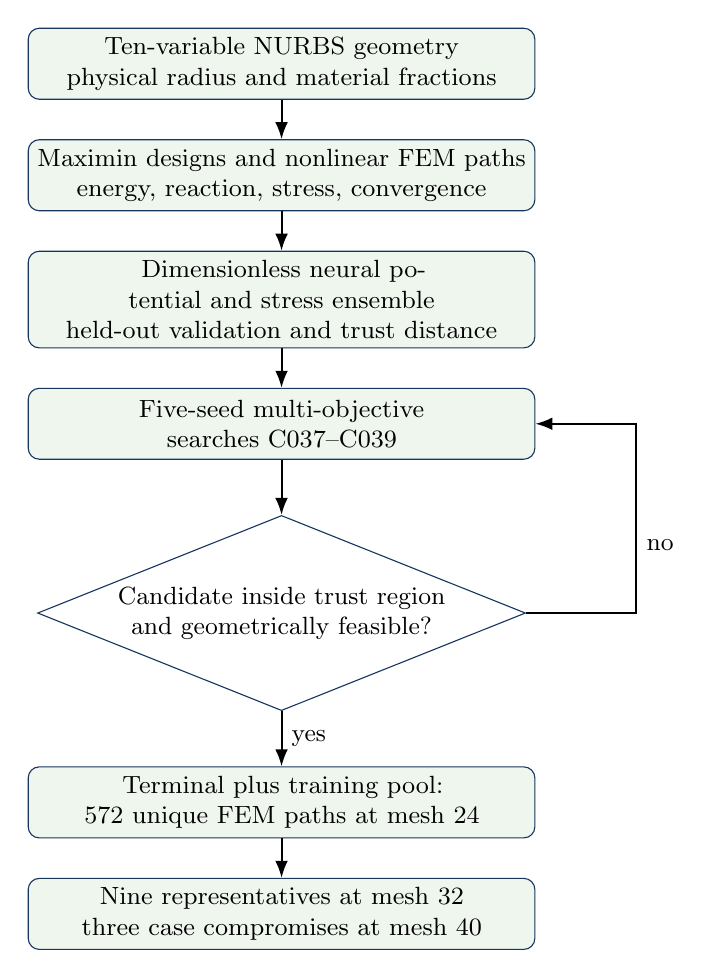
\begin{tikzpicture}[node distance=5mm,>=Latex,font=\small,
block/.style={draw=engblue,rounded corners,align=center,minimum height=9mm,text width=62mm,fill=enggreen!45},
decision/.style={draw=engblue,diamond,aspect=2.5,align=center,inner sep=1.5pt,fill=white},
arrow/.style={->,line width=0.7pt}]
\node[block] (g) {Ten-variable NURBS geometry\\physical radius and material fractions};
\node[block,below=of g] (f) {Maximin designs and nonlinear FEM paths\\energy, reaction, stress, convergence};
\node[block,below=of f] (n) {Dimensionless neural potential and stress ensemble\\held-out validation and trust distance};
\node[block,below=of n] (o) {Five-seed multi-objective searches C037--C039};
\node[decision,below=7mm of o] (d) {Candidate inside trust region\\and geometrically feasible?};
\node[block,below=7mm of d] (v) {Terminal plus training pool:\\572 unique FEM paths at mesh 24};
\node[block,below=of v] (m) {Nine representatives at mesh 32\\three case compromises at mesh 40};
\draw[arrow] (g)--(f); \draw[arrow] (f)--(n); \draw[arrow] (n)--(o);
\draw[arrow] (o)--(d); \draw[arrow] (d)--node[right]{yes}(v); \draw[arrow] (v)--(m);
\draw[arrow] (d.east)--++(14mm,0)|-node[pos=0.18,right]{no}(o.east);
\end{tikzpicture}
\caption{Computation and verification workflow. The neural layer proposes designs; direct finite-element solutions determine every mechanical quantity and pooled-candidate nondominated classification, with targeted refinement of selected members.}
\label{fig:workflow}
\end{figure}

\section{Geometric design model}

\subsection{Decision variables and rational profile}

The coupled vector is
\begin{equation}
\bm x=(x_1,\ldots,x_5,x_6,x_7,P,H,t)\in\mathbb R^{10},
\label{eq:vector}
\end{equation}
with bounds
\begin{align}
x_{1:5}&\in[0.1,10], & x_{6:7}&\in[0,1],\nonumber\\
P&\in[4.8,7.9]\;\text{mm}, & H&\in[2.2,4.0]\;\text{mm},\nonumber\\
t&\in[0.15,0.25]\;\text{mm}. &&
\label{eq:bounds}
\end{align}
The first five positive variables are normalized,
\begin{equation}
d_i=\frac{x_i}{\sum_{j=1}^{5}x_j},\qquad i=1,\ldots,5,
\end{equation}
so common scaling of $x_{1:5}$ does not change the geometry. They define ten control-point abscissae over two normalized periods,
\begin{align}
X=&[0,d_1,d_1+d_2,d_1+d_2+d_3,d_1+\cdots+d_4,\nonumber\\
&1+d_1,1+d_1+d_2,1+d_1+d_2+d_3,\nonumber\\
&1+d_1+\cdots+d_4,2],
\end{align}
with ordinates $Y=[0,0,1,1,0,0,1,1,0,0]$. The rational factors are
\begin{equation}
r_k=0.0103\exp(9.17x_{5+k})+0.1,\qquad k=1,2,
\label{eq:weight_mapping}
\end{equation}
and the weights are $\bm w=[1,r_1,r_1,r_2,r_2,r_1,r_1,r_2,r_2,1]$. A clamped uniform degree-two knot vector completes the curve definition. The sampling grid includes $u=1/4$, $1/2$, and $3/4$ exactly. The crown-to-crown interval $u\in[1/4,3/4]$ is the mechanical cell; its endpoint ordinates and tangents agree, so the extracted geometry is $C^1$ periodic before independent affine maps impose $P$ and $H$.

Figure~\ref{fig:param} shows how the study moves from size-only and control-point families to the compact coupled representation. The ten-variable form retains enough freedom to change crown flatness and transition curvature while allowing exact size bounds and a manageable feasible region.

\begin{figure}[t]
\centering
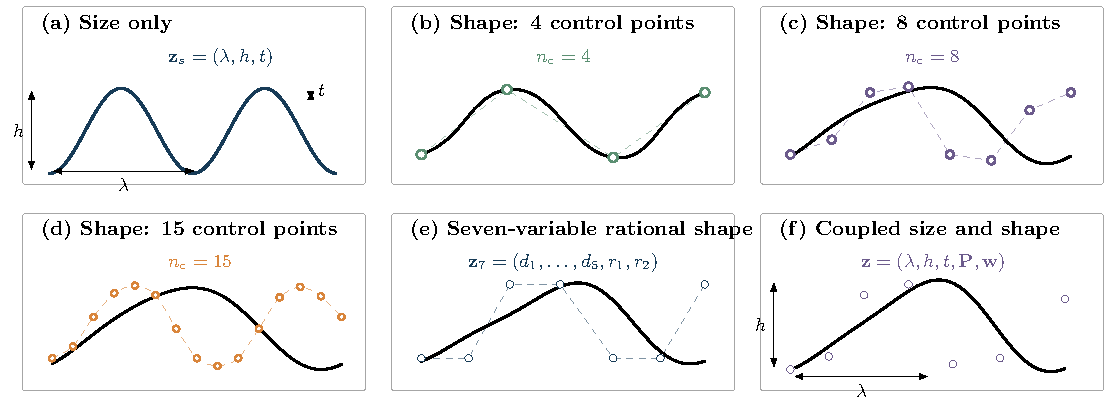
\includegraphics[width=0.96\textwidth]{optimization_parameterizations.pdf}
\caption{Geometric parameterizations considered in the geometric benchmark. The nonlinear mechanical campaigns use the compact seven-variable rational profile augmented by pitch, height, and thickness.}
\label{fig:param}
\end{figure}

\subsection{Physical profile, arc length, and curvature}

For control points $\bm P_i$ and quadratic basis $N_{i,2}$, the rational basis and centreline are
\begin{equation}
R_i(u)=\frac{w_iN_{i,2}(u)}{\sum_jw_jN_{j,2}(u)},\qquad
\bm c(u)=\sum_iR_i(u)\bm P_i.
\label{eq:nurbs}
\end{equation}
After physical scaling, the period arc length is
\begin{equation}
L_s=\int_{u_a}^{u_b}\sqrt{x'(u)^2+y'(u)^2}\,\mathrm du.
\label{eq:arc}
\end{equation}
The geometric evaluator uses at least 800 physical-curve samples for selection and reporting, while retaining the three exact cell-defining parameters. Curvature is obtained from first and second numerical gradients with a fixed Gaussian regularization applied identically to every profile,
\begin{equation}
\kappa=\frac{|x'y''-y'x''|}{(x'^2+y'^2)^{3/2}},\qquad
\Rmin=\frac{1}{\max\kappa}.
\label{eq:curvature}
\end{equation}
The manufacturing constraint is
\begin{equation}
g_R=\max(0,0.9-R_1)+\max(0,0.9-R_2)=0,
\label{eq:radius_constraint}
\end{equation}
where $R_1$ and $R_2$ are limiting radii in the two transition zones. For FEM, the exact $u\in[1/4,3/4]$ cell is retained in curve order rather than sorted on $x$. The two periodic crowns and central trough are mandatory nodes, and remaining nodes are distributed by arc length within the two intervening branches. Thus every resolution preserves near-vertical portions, identical endpoint ordinates and tangents, and zero initial free travel at both platens. Across all 1200 profiles in the feasible cloud, the computed endpoint-ordinate gap is identically zero at floating-point precision and the largest unit-tangent mismatch is $3.04\times10^{-14}$.

\begin{table}[t]
\centering\small
\caption{Numerical periodicity audit over the complete feasible design cloud. Unit tangents use centered differences on a grid containing both cell endpoints exactly.}
\label{tab:periodicity_audit}
\begin{tabular}{lr}
\toprule
Quantity & Value \\
\midrule
Profiles checked & 1200 \\
Largest endpoint-ordinate gap [mm] & 0.000e+00 \\
Largest unit-tangent mismatch & 3.035e-14 \\
\bottomrule
\end{tabular}
\end{table}


\subsection{Geometric board quantities}

For a unit out-of-plane width, the corrugated medium contributes $tL_s$ of material area per period. With two liners of the same thickness, the board material fraction within the bounding rectangle is
\begin{equation}
\phib=\frac{t(L_s+2P)}{PH},
\qquad
\phic=\frac{tL_s}{PH}
\label{eq:material_fraction}
\end{equation}
for the complete board proxy and core-only fraction, respectively. The geometric benchmark also evaluates material area per wavelength, second moment per wavelength, and an effective linear transverse modulus. The section quantities follow
\begin{align}
A&=\int t\,\mathrm ds+2Pt,\nonumber\\
\bar y&=\frac{1}{A}\int y\,\mathrm dA,\nonumber\\
I&=\int (y-\bar y)^2\,\mathrm dA,
\end{align}
including two liner contributions for $A$ and $I$. Orientation-dependent paper compliance is rotated along the local tangent before period integration to obtain the diagnostic $E_{z,\mathrm{eff}}$. These quantities remain geometric or linear-elastic proxies; they are not identified with nonlinear crush strength.

\section{Nonlinear finite-element compression model}

\subsection{Scope and boundary protocol}

The mechanical calculation represents one stress-free, pre-formed corrugated medium between rigid horizontal surfaces. The surfaces idealize rigid liners. Their local normal attachments are kinematic: the central trough follows the stationary lower surface, while the two periodic crown nodes share vertical displacement and rotation and follow the moving upper surface. Flexible liner bending, adhesive constitutive thickness, debonding, and friction are not resolved. Physical liner surfaces are placed one half-thickness outside the initial centreline extrema, at $-t/2$ and $H+t/2$, so equivalent centreline bounds are $0$ and $H$ initially. Tangential slip is free: the left crown supplies the horizontal gauge, while the horizontal period can contract through the right-crown degree of freedom. All other nodes retain unilateral vertical bounds and cannot cross either surface. Surface resultants are signed sums over constrained roots: a local normal-attachment contribution opposing the net compression is retained rather than clipped.

The load parameter is engineering platen-travel strain
$\epsilon=\delta/H=[(H+t)-H_p]/H$, where $\delta$ is upper-platen travel and $H_p$ is current physical surface separation. Thus the $t/2$ surface offsets define contact geometry without changing the prescribed travel $\delta=\epsilon H$. Every path uses
\begin{equation}
\epsilon\in\{0,0.05,0.10,0.15,0.20\},
\label{eq:path}
\end{equation}
with continuation from the previous converged displacement. The material and section parameters are listed in Table~\ref{tab:fem_protocol}.

\begin{table}[t]
\centering\small
\caption{Nonlinear FEM and optimization protocol.}
\label{tab:fem_protocol}
\begin{tabularx}{\textwidth}{lX}
\toprule
Quantity & Value or rule \\
\midrule
Longitudinal modulus $E$ & 2899 MPa \\
Shear modulus $G$ & $E/55$ \\
Yield stress $\sigma_y$ & 60 MPa \\
Hardening ratio & 0.02 \\
Out-of-plane width $b$ & 25 mm \\
Training mesh & 16 elements per period \\
Complete reconstruction mesh & 24 elements per period \\
Representative check mesh & 32 elements per period \\
Compromise refinement mesh & 40 elements per period \\
Path & Eq.~\eqref{eq:path} \\
Solver & L-BFGS-B; alternate SLSQP solution of the same energy and KKT check \\
Radius threshold & 0.9 mm \\
Neural-potential seeds & 3, 11, 29, 47, 83 \\
Optimizer seeds & 3, 11, 29, 47, 83 \\
Swarm size; generations & 36; 56 \\
\bottomrule
\end{tabularx}
\end{table}

The fixed nominal values in Table~\ref{tab:fem_protocol} isolate geometric effects in this study; they are not calibrated to a particular commercial paper grade.

\subsection{Corotational beam energy}

Each node carries global translations and a section rotation. For element $e$ of initial length $L_e$, the corotated axial extension is $\Delta L_e$ and the end rotations relative to the current chord are $\theta_{1e}$ and $\theta_{2e}$. The constant assumed strains are
\begin{equation}
\varepsilon_{0e}=\frac{\Delta L_e}{L_e},\qquad
\kappa_e=\frac{\theta_{2e}-\theta_{1e}}{L_e},\qquad
\gamma_e=\frac{\theta_{1e}+\theta_{2e}}{2}.
\label{eq:assumed_strains}
\end{equation}
The element deformation energy used in both elastic and smoothly yielding calculations is
\begin{equation}
\Pi_e=bL_e\int_{-t/2}^{t/2}
W_f(\varepsilon_{0e}-\kappa_e z)\,\mathrm dz
+\frac{1}{2}k_sGA L_e\gamma_e^2,
\qquad A=bt,\quad k_s=\frac{5}{6}.
\label{eq:beam_energy}
\end{equation}
The thickness integral is evaluated by five-point Gauss quadrature, whereas the constant mean shear strain is integrated once. This assumed/reduced shear treatment avoids locking of a fully integrated two-node shear field. In the small-strain elastic limit it recovers the expected axial, bending, and mean-shear energies. Large rotations enter through the current chord, so the model is geometrically nonlinear \citep{Crisfield1991}. The same scalar energy in Eq.~\eqref{eq:beam_energy} is differentiated by automatic differentiation for equilibrium and post-processing; no alternative condensed stiffness expression is used. Unilateral bounds are handled directly in constrained minimization, avoiding a contact penalty. Active-set interpretation follows standard nonlinear contact mechanics \citep{Wriggers2006}.

If $\varepsilon_f=\varepsilon_{0e}-\kappa_ez$ is longitudinal fibre strain and $q=E\varepsilon_f/\sigma_y$, the smooth density is
\begin{equation}
W_f=h_r\frac{E\varepsilon_f^2}{2}
+(1-h_r)\frac{E\varepsilon_f^2}{\sqrt{1+q^2}+1},
\label{eq:smooth_yield}
\end{equation}
with hardening ratio $h_r=0.02$. The law approaches linear elasticity near zero, saturates toward the declared yield level, and retains a small tangent. It is a deformation-potential regularization, not an incremental damage or dissipation model. Consequently, terminal potential is called stored potential, not absorbed crash energy.

\subsection{Reaction, work, stress, and solver acceptance}

The top reaction $F$ is recovered from active unilateral constraints. Reaction-integrated external work is evaluated independently,
\begin{equation}
W=\int_0^{0.2H}F(\delta)\,\mathrm d\delta,
\label{eq:external_work}
\end{equation}
using the five path states. Extreme-fibre stresses are recovered at both ends of every element. Search-stage stress uses a length-weighted $p$-norm with $p=8$,
\begin{equation}
\sigma_{8}=\left(
\frac{\sum_eL_e\sigma_e^8}{\sum_eL_e}
\right)^{1/8},
\label{eq:stress_pnorm}
\end{equation}
where $\sigma_e$ is the maximum absolute extreme-fibre stress in element $e$. Length-weighted 99th-percentile and raw maximum stresses are retained for verification.

A state satisfies the numerical equilibrium check when
\begin{equation}
\frac{\lVert\bm g_{\mathrm{proj}}\rVert_\infty}{\sigma_ybt}
\leq5\times10^{-4},
\label{eq:solver_acceptance}
\end{equation}
where $\bm g_{\mathrm{proj}}$ is the bound-aware projected gradient. Raw L-BFGS-B success and this check accept the primary state. If the primary flag is negative, the same bound-constrained energy is minimized by the alternate SLSQP optimization algorithm from the primary endpoint; this is an algorithmic cross-check, not an independent mechanical model. The fallback must return raw success and satisfy the same projected-KKT threshold. If neither algorithm does so, the load interval is retried with 2, 4, and then 8 subdivisions. A path is accepted only if all published load states pass one of the two algorithms. Signed surface resultants provide an independent dimensionless force-balance audit,
\begin{equation}
\mathcal E_R=\max_{\epsilon>0}
\frac{|F_{\mathrm{upper}}(\epsilon)-F_{\mathrm{lower}}(\epsilon)|}
{\sigma_ybt}.
\label{eq:reaction_balance}
\end{equation}
The ledgers preserve the primary and fallback status, messages, iteration counts, projected gradients, upper and lower reactions, $\mathcal E_R$, contact positions, subdivision count, and protocol fingerprint. Exceptions, non-finite states, failed paths, radius violation, and trust-region violation receive dominated objectives plus continuous constraint violation rather than being silently discarded.

\section{Dimensionless formulation}

\subsection{Input and manufacturing groups}

Only independent groups are used as neural inputs. Because $\sum_i d_i=1$, $d_5$ is determined by the first four spacings. With the two rational-weight parameters $x_6,x_7$, the eight-entry geometric basis is
\begin{equation}
\bm z_g=\left(d_1,d_2,d_3,d_4,x_6,x_7,
\eta,\tau_H\right),
\quad
\eta=\frac{H}{P},\quad
\tau_H=\frac{t}{H}.
\label{eq:input_groups}
\end{equation}
The state coordinate is $\epsilon$, while $G/E$ and $\sigma_y/E$ are fixed material parameters. Curvature and pitch slenderness remain useful derived reports,
\begin{equation}
\tau_P=\frac{t}{P}=\eta\tau_H,\qquad
\Pi_\kappa=\frac{t}{\Rmin},\qquad
\mathcal C_y=\frac{t/(2\Rmin)}{\sigma_y/E}
=\frac{E}{2\sigma_y}\Pi_\kappa.
\label{eq:derived_groups}
\end{equation}
The final relation compares nominal outer-fibre forming strain with elastic yield strain. Both $\Pi_\kappa$ and $\mathcal C_y$ are deterministic functions of the eight independent descriptors and the fixed material ratio, so they are manufacturing-severity reports rather than additional neural coordinates or objectives.
The pre-formed geometry is taken as stress free in the service-load model, so $\mathcal C_y$ is not a residual-stress prediction.

\subsection{Mechanical response numbers}

The terminal load and potential are normalized by yield-scale section quantities,
\begin{align}
C_F&=\frac{F}{\sigma_ybt},\label{eq:load_number}\\
\PsiU&=\frac{U}{\sigma_ybtL_s},\label{eq:potential_number}\\
\PsiW&=\frac{W}{\sigma_ybtL_s}.\label{eq:work_number}
\end{align}
Stress utilization, localization, and last-interval tangent are
\begin{align}
\Om&=\frac{\sigma_8}{\sigma_y},
&\Omega_{99}&=\frac{\sigma_{99,L}}{\sigma_y},
&\Ommax&=\frac{\sigma_{\max}}{\sigma_y},\label{eq:stress_numbers}\\
\mathcal L_\sigma&=\frac{\sigma_{99,L}bt}{F},
&\Theta&=\frac{H}{Ebt}\frac{\Delta F}{\Delta\delta}.
\label{eq:localization_tangent}
\end{align}
The tangent is a scalar path indicator over the 15--20\% interval; it is not a complete stability eigenvalue.

Three dimensionless selectors are introduced for ranking an already computed front,
\begin{equation}
\mathcal I_{WM}=\frac{\PsiW}{\phib},\qquad
\mathcal I_{WS}=\frac{\PsiW}{\Om},\qquad
\Iws=\frac{\PsiW}{\phib\Om}.
\label{eq:selectors}
\end{equation}
They are not additional optimization objectives because they are algebraically correlated with existing quantities. They provide a compact way to compare work per material, work per stress utilization, and their combined balance.

\begin{table}[t]
\centering\small
\caption{Dimensionless response dictionary and use in the study.}
\label{tab:dimensionless_dictionary}
\begin{tabularx}{\textwidth}{lXll}
\toprule
Quantity & Interpretation & Search use & Direction \\
\midrule
$\phic$ & medium material fraction & report & minimize \\
$\phib$ & medium plus two-liner material proxy & objective/constraint & minimize \\
$\mathcal C_y$ & forming strain relative to yield strain & report & lower \\
$C_F$ & crush reaction relative to yield load & report & higher \\
$\PsiU$ & terminal stored potential & neural screen/FEM objective & higher \\
$\PsiW$ & reaction-integrated external work & FEM report & higher \\
$\Om$ & smooth length-weighted stress utilization & objective & minimize \\
$\Omega_{99}$ & robust local stress indicator & verify & lower \\
$\Ommax$ & raw peak stress & mesh study & lower \\
$\mathcal L_\sigma$ & local-to-nominal stress concentration & report & lower \\
$\Theta$ & last-interval dimensionless tangent & verify & positive \\
$\mathcal E_R$ & signed surface-force imbalance/yield load & solver audit & lower \\
$\Iws$ & work/material/stress selector & shortlist & higher \\
\bottomrule
\end{tabularx}
\end{table}

\section{Energy-consistent neural potential and stress screen}

\subsection{FEM design set}

The coupled geometric populations define feasible starting neighborhoods. Local multiplicative perturbations of $x_{1:5}$ and additive perturbations of weights and size variables create a cloud of 1200 profiles. Each is re-evaluated at 800 curve samples and retained only if $\Rmin\ge0.905$~mm. Descriptors are standardized, and farthest-point sampling selects 80 designs that span the cloud. Every fourth selected design is held out, producing 60 training and 20 test geometries. Because all five load states from one geometry remain in the same split, the test does not leak adjacent states from a training geometry.

The neural descriptor is exactly Eq.~\eqref{eq:input_groups}: four independent normalized spacings, two rational-weight variables, $H/P$, and $t/H$. The last network input is normalized strain $\bar\epsilon=\epsilon/0.25$. The derived curvature ratio is deliberately omitted so it cannot redundantly reweight the standardized trust distance. Fixed material ratios $G/E$ and $\sigma_y/E$ are omitted because they do not vary in this study.

\subsection{Energy-consistent architecture}

The neural potential uses two tanh hidden layers of 14 units. Let $s_\Psi$ be the 95th percentile of training-set $\Psi_U$. Its dimensionless output is parameterized as
\begin{equation}
\frac{\widehat\Psi_U(\bm z,\bar\epsilon)}{s_\Psi}
=\bar\epsilon^2\operatorname{softplus}[g_{\bm\theta}(\bm z,\bar\epsilon)],
\label{eq:energy_architecture}
\end{equation}
which imposes zero potential and zero force at zero compression and prevents negative potential. The conjugate dimensionless force is obtained by differentiation,
\begin{equation}
\widehat q_F=\frac{\partial\widehat\Psi_U}{\partial\epsilon}
=\frac{FH}{\sigma_ybtL_s}.
\label{eq:force_conjugacy}
\end{equation}
For adjacent path states, define the predicted secant conjugate force $\widehat{\bar q}_{F,k}=(\widehat\Psi_{U,k}-\widehat\Psi_{U,k-1})/(\epsilon_k-\epsilon_{k-1})$ and let $\bar q_{F,k}$ be the corresponding average of the two FEM reactions after the scaling in Eq.~\eqref{eq:force_conjugacy}. With $s_q$ equal to the 95th percentile of the training conjugate forces, the loss combines scaled potential error, average-reaction error, a non-negative-reaction penalty, and mean parameter regularization,
\begin{align}
\mathcal J(\bm\theta)=&\frac{1}{N}\sum_i
\left(\frac{\widehat\Psi_{U,i}-\Psi_{U,i}}{s_\Psi}\right)^2
+\frac{1}{N_p}\sum_k
\left(\frac{\widehat{\bar q}_{F,k}-\bar q_{F,k}}{s_q}\right)^2\nonumber\\
&+\frac{2}{N_p}\sum_k
\left[\frac{\max(-\widehat{\bar q}_{F,k},0)}{s_q}\right]^2
+\frac{10^{-3}}{N_\theta}\|\bm\theta\|_2^2.
\label{eq:energy_loss}
\end{align}
Five networks with seeds 3, 11, 29, 47, and 83 form an ensemble. All reach the predeclared 900-iteration L-BFGS-B cap; held-out error, not optimizer termination text, determines model acceptance. The five parameter sets are serialized separately so predictions can be reproduced without retraining.

\subsection{Stress emulator and trust distance}

Local stress is not derived from the global neural potential. A separate 160-tree extra-trees ensemble maps the same eight geometry descriptors to terminal $\Om$. Let $\overline\Omega_{\mathrm{tree}}$ denote its tree-average prediction. For descriptive error calibration only, define
\begin{equation}
\widehat\Om_{c}=\overline\Omega_{\mathrm{tree}}+\Delta\Omega,
\qquad \Delta\Omega=0.01706,
\label{eq:conservative_stress}
\end{equation}
where $\Delta\Omega$ is the higher-method 90th percentile of held-out residuals $\Omega_8-\overline\Omega_{\mathrm{tree}}$. It covers 19 of 20 held-out targets (95\% empirical coverage). Because an additive constant changes neither within-case ranks nor nondominated membership, the optimization uses the unshifted mean $\overline\Omega_{\mathrm{tree}}$; $\Delta\Omega$ is not presented as an optimization safeguard. The same 20 designs supply the reported test metrics, so coverage is descriptive rather than an independent generalization estimate. The ensemble, feature scaler, and nearest-neighbor model are serialized. This stress model is explicitly statistical rather than mechanically constrained.

For each candidate, standardized nearest-neighbor distance $D$ to the 60 training designs is computed. The trust limit is
\begin{equation}
D_{\max}=1.5Q_{0.95}(D_{\mathrm{LOO}})=2.918,
\label{eq:trust}
\end{equation}
where $D_{\mathrm{LOO}}$ is the training leave-one-out nearest-neighbor distance. A candidate outside this region is infeasible even if its predicted objectives appear attractive.

\section{Multi-objective optimization and FEM reconstruction}

\subsection{Three physics cases}

The new problems use minimization coordinates:
\begin{align}
\mathrm{C037}:&\quad \min(\phib,1/\widehat\Psi_U),\label{eq:c037}\\
\mathrm{C038}:&\quad \min(\phib,\overline\Omega_{\mathrm{tree}}),
\quad \widehat\Psi_U\ge4.555\times10^{-4},\label{eq:c038}\\
\mathrm{C039}:&\quad \min(1/\widehat\Psi_U,\overline\Omega_{\mathrm{tree}}),
\quad \phib\le0.217537.
\label{eq:c039}
\end{align}
All cases also enforce Eqs.~\eqref{eq:radius_constraint} and \eqref{eq:trust}. The C038 potential floor is the 40th percentile and the C039 material cap is the 65th percentile of the 60 training designs; held-out designs and optimizer outputs do not set either threshold. C037 exposes the broad material--mechanical envelope. C038 asks how stress can be reduced while retaining a lower-quantile potential. C039 isolates the potential--stress exchange under a material cap. Alternative training quantiles are evaluated after optimization to expose threshold dependence.

\subsection{Seeded MO-ETPSO}

Random sampling in the complete ten-dimensional box yields very few radius-feasible shapes. Each run is therefore initialized from 36 feasible maximin or coupled designs. A small initial velocity, 2.5\% of each variable range, avoids immediately leaving the feasible manifold. The swarm uses inertia $0.7$, $c_1=c_2=2.05$, a constriction factor, standard Pareto domination, normalized crowding, and continuous constraint violation. Five seeds and 56 generations give $36\times56=2016$ surrogate calls per run and 15 runs in total. A fixed hypervolume reference is used within each case. Complete terminal populations are pooled by case, duplicates are removed, and surrogate nondomination is recalculated across seeds; terminal populations themselves are retained for direct verification.

\subsection{Direct mechanical reconstruction}

All 540 terminal particles are considered, not only the surrogate-nondominated subset. The 80 FEM designs are also classified under every case and merged with the terminal populations. Exact case--vector deduplication leaves 732 classifications representing 572 unique geometries. Each unique geometry is solved once along the complete path at 24 elements per wavelength, after which its raw mechanical record is reclassified under every applicable case. This larger universe prevents the optimizer trajectory alone from defining direct nondomination; in particular, a training design can displace a terminal point.

Direct objectives replace $\widehat\Psi_U$ and $\overline\Omega_{\mathrm{tree}}$ with $\PsiU$ and $\Om$; solver and case constraints are recomputed from raw mechanics. Pareto membership is then reconstructed separately for C037, C038, and C039 by exact pairwise minimization over successful, case-feasible mesh-24 classifications. The CSV round trip is joined with a ten-coordinate geometry key rounded to ten decimals rather than raw binary floating-point equality. The code asserts one mechanics record for every classification and rejects any missing match before dominance is evaluated. This safeguard is consequential: a missing Boolean cannot be interpreted as a successful path.

Within each pooled-candidate nondominated set, the two objective extremes and the point nearest the normalized utopia point are selected. All nine unique representatives are re-solved at 32 elements per wavelength. The three case compromises are also solved at 40 elements and supply the refined stress-field figures. For any response $q$, the reported paired mesh change from level $a$ to finer level $b$ is
\begin{equation}
\delta_{a\rightarrow b}(q)=
\frac{|q_b-q_a|}{\max(|q_b|,10^{-12})},
\label{eq:mesh_change}
\end{equation}
so the finer-mesh value is the denominator. The 24--32 changes measure the complete representative set; the 32--40 changes provide a finer check on one central trade-off per case. Three exploratory 48-element paths reached optimizer iteration limits at one or more substeps and failed the predeclared strict path criterion; their values are excluded from every table, figure, nondominated set, and conclusion. Mechanics caches are keyed by rounded geometry coordinates and full protocol fingerprints. The execution manifest binds the fixed 9+3 verification budget, all effective source and trained-model files, numerical inputs and outputs, and every table and figure included in the manuscript using SHA-256 hashes. A separate two-state mesh-8 path is used only for the formulation check in Table~\ref{tab:formulation_verification}; it is not a design candidate.

\begin{table}[t]
\centering
\caption{Mechanical evidence budget. Case classifications share mechanics when their ten-variable vectors coincide.}
\label{tab:verification_pool_fast}
\begin{tabular}{lr}
\toprule
Evidence set & Count \\
\midrule
Direct case classifications at mesh 24 & 732 \\
Unique mesh-24 mechanical geometries & 572 \\
Representative mesh-32 geometries & 9 \\
Compromise mesh-40 geometries & 3 \\
\bottomrule
\end{tabular}
\end{table}


\section{Geometric benchmark results}

Before introducing nonlinear objectives, the geometric evaluator and optimizer are assessed on the fixed seven-variable shape problem. Material area per wavelength is minimized against reciprocal inertia under the 0.9~mm radius constraint. MO-ETPSO and NSGA-II use equal populations, 4000 evaluator calls, and ten paired seeds. Using the fixed reference $(1,15)$ in the scaled optimization coordinates, mean final hypervolume is 4.0206 for MO-ETPSO and 4.0136 for NSGA-II; the paired Wilcoxon result is $p=0.105$. Thus the fixed terminal experiment does not support a statistically resolved difference, although the swarm exhibits lower run-to-run variation and earlier median envelope discovery.

Both pooled algorithms occupy the narrow band
\begin{equation}
A/P=1.723\text{--}1.794~\mathrm{mm},\qquad
I/P=3.936\text{--}4.094~\mathrm{mm^3}.
\end{equation}
Figure~\ref{fig:geometric_front} reports fronts and convergence. Figure~\ref{fig:geometric_selected} shows that visible shape changes remain possible within a narrow pair of global geometric objectives, motivating the nonlinear extension.

\begin{figure}[t]
\centering
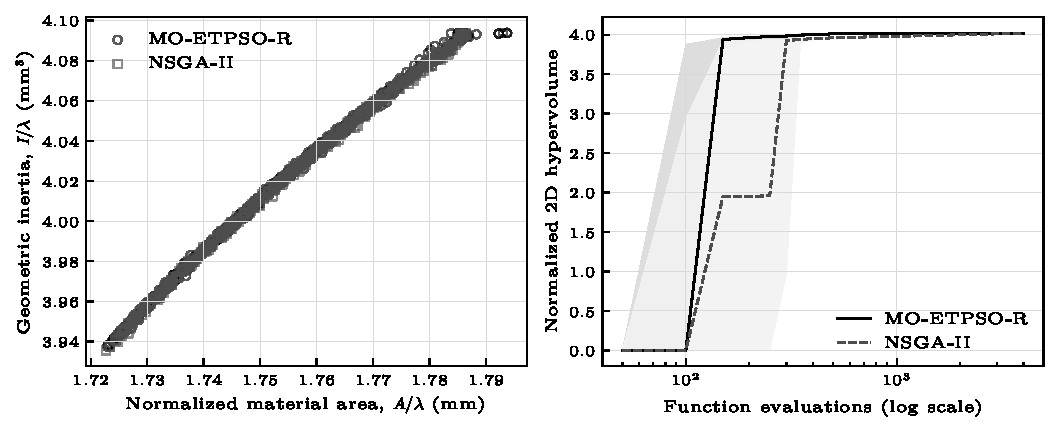
\includegraphics[width=0.95\textwidth]{pareto_and_convergence.pdf}
\caption{Equal-budget geometric benchmark. Pareto coordinates are evaluated in physical units after optimization; convergence is reported over paired seeds.}
\label{fig:geometric_front}
\end{figure}

\begin{figure}[t]
\centering
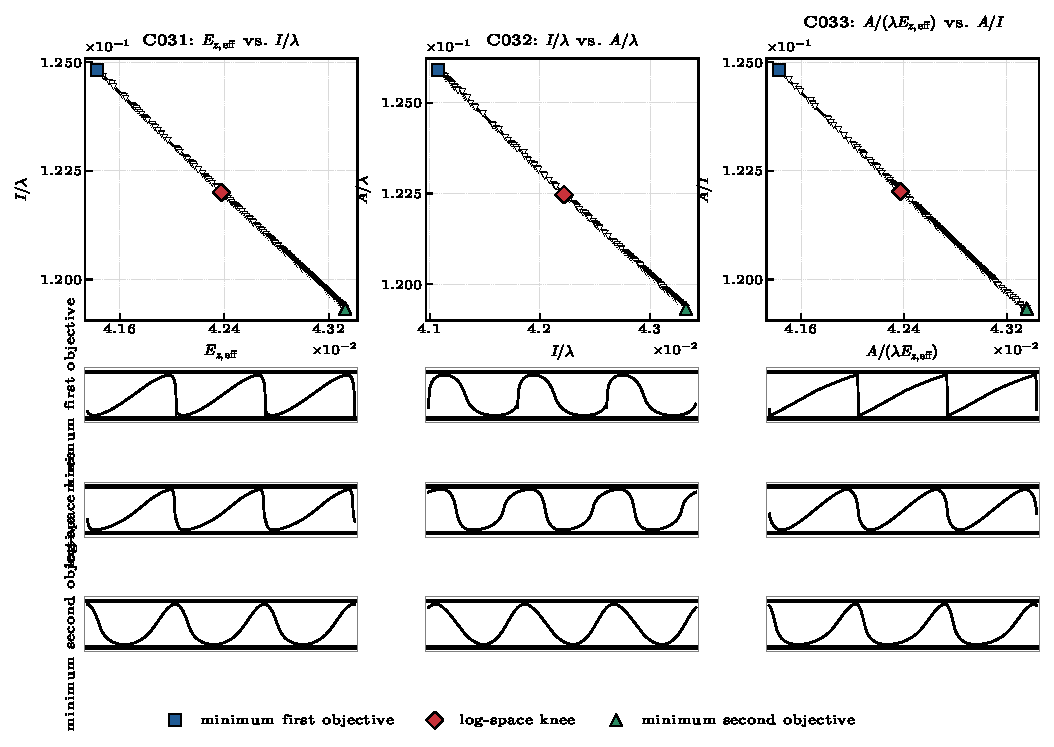
\includegraphics[width=\textwidth]{constrained_selected_designs.pdf}
\caption{Representative radius-feasible geometric designs. Similar area--inertia performance does not imply the same local curvature or nonlinear compression response.}
\label{fig:geometric_selected}
\end{figure}

The broader parameterization study is summarized in Fig.~\ref{fig:atlas}. Size-only, shape-only, and coupled cases create different objective envelopes. These results remain geometric baselines, while C037--C039 replace dimensional scalings with Eqs.~\eqref{eq:c037}--\eqref{eq:c039}.

\begin{figure}[p]
\centering
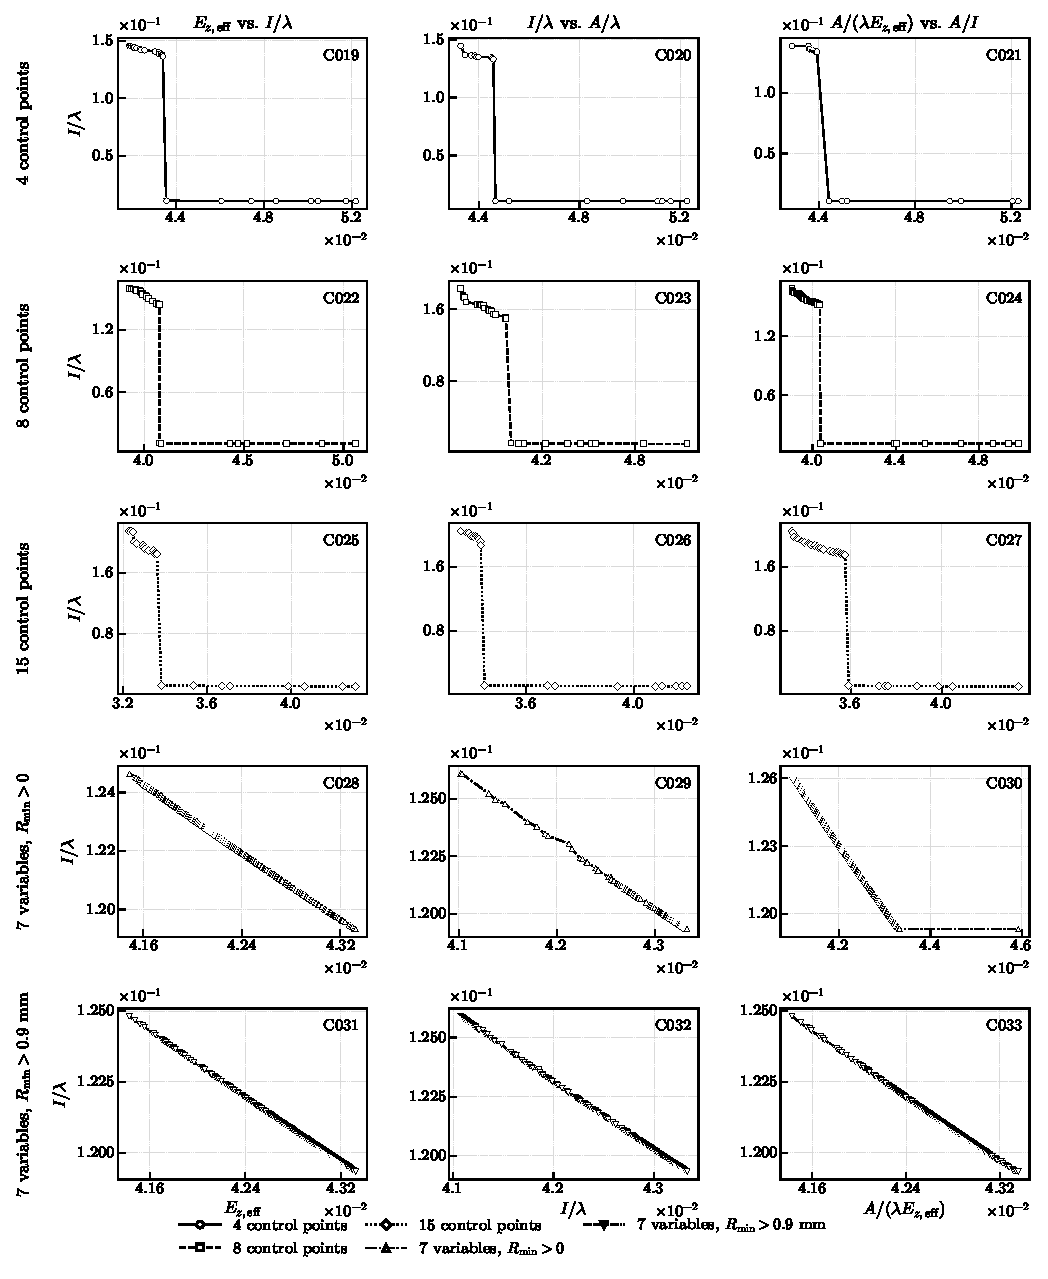
\includegraphics[width=0.98\textwidth]{pareto_atlas_5x3.pdf}
\caption{Geometric case atlas across size and shape parameterizations. The atlas establishes the diversity available before nonlinear mechanical screening.}
\label{fig:atlas}
\end{figure}

\FloatBarrier
\section{FEM and surrogate validation results}

All 80 selected geometries complete their five-state 16-element paths, giving 400 accepted states. Figure~\ref{fig:validation} compares held-out predictions with FEM. Across the complete path, the five-network ensemble attains $R^2=0.984$ for dimensional potential, $0.982$ for potential number, and $0.982$ for reaction. The terminal stress model attains $R^2=0.885$. Table~\ref{tab:physics_validation} reports both path-level and 20\% target-state validation without mixing geometries across the split.

\begin{figure}[H]
\centering
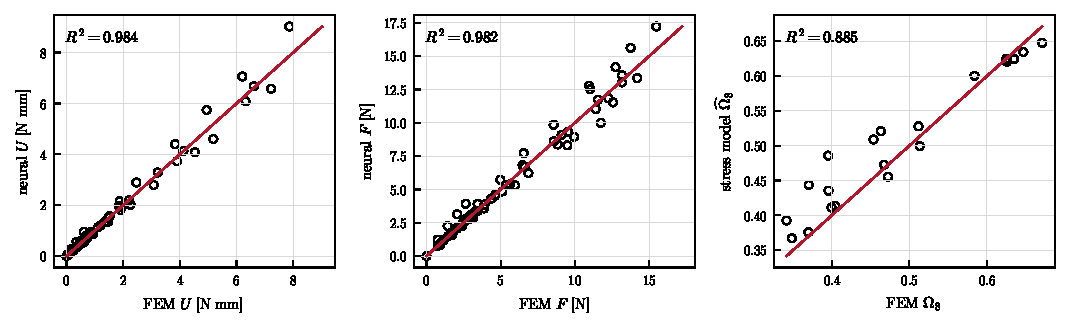
\includegraphics[width=0.97\textwidth]{fem_energy_surrogate_validation.pdf}
\caption{Held-out design-level validation for potential, reaction, and smooth stress utilization. The diagonal is equality. The stress panel is an auxiliary tree ensemble; the first two panels come from the differentiated neural potential.}
\label{fig:validation}
\end{figure}

\begin{table*}[t]
\centering\small
\caption{Held-out design-level validation. Relative error is the mean absolute relative error; near-zero states are excluded from the path-level relative-error statistic.}
\label{tab:physics_validation}
\begin{tabular}{lllrr}
\toprule
Response & Model & Scope & $R^2$ & Rel. error \\
\midrule
Dimensional potential $U$ & structured energy surrogate & complete path & 0.984 & 7.0\% \\
Potential number $\Psi_U$ & structured energy surrogate & complete path & 0.982 & 7.4\% \\
Compression reaction $F$ & energy derivative & complete path & 0.982 & 7.1\% \\
Stress utilization $\Omega_8$ & tree ensemble & 20\% strain & 0.885 & 6.3\% \\
\bottomrule
\end{tabular}
\end{table*}


\begin{table}[t]
\centering\small
\caption{Fixed-budget energy-surrogate fits. All seeds use the same 900-iteration cap; scientific acceptance is based on geometry-held-out response error rather than the optimizer termination flag.}
\label{tab:energy_training}
\begin{tabular}{rrrl}
\toprule
Seed & Iterations & Final loss & Termination \\
\midrule
3 & 900 & 8.876e-05 & gradient iteration cap \\
11 & 900 & 8.212e-05 & gradient iteration cap \\
29 & 900 & 8.884e-05 & gradient iteration cap \\
47 & 900 & 8.563e-05 & gradient iteration cap \\
83 & 900 & 9.212e-05 & gradient iteration cap \\
\bottomrule
\end{tabular}
\end{table}


Path-level mean relative errors are 7.0\% for potential and 7.1\% for reaction after excluding near-zero states; terminal stress mean relative error is 6.3\%. These errors support in-domain screening but not final ranking near a Pareto front. Table~\ref{tab:stress_calibration} reports the additive residual diagnostic and explains why it does not alter the optimizer.

\begin{table}[t]
\centering\small
\caption{Descriptive additive stress calibration on the 20 held-out designs. The constant is reported as an error diagnostic; because it preserves every within-case rank, the optimizer uses the unshifted ensemble mean.}
\label{tab:stress_calibration}
\begin{tabular}{lr}
\toprule
Quantity & Value \\
\midrule
Target empirical coverage & 90\% \\
Diagnostic margin $\Delta\Omega$ & 0.01706 \\
Observed empirical coverage & 95\% \\
Largest residual underprediction after shift & 0.00640 \\
\bottomrule
\end{tabular}
\end{table}


The custom element implementation is checked independently of the design campaign in Table~\ref{tab:formulation_verification}. Constant-shear and pure-bending states are compared with their closed-form Timoshenko energies, and the automatic energy gradient is compared with a centred finite difference. A small two-state, eight-element corrugated contact path then checks zero initial platen gap, reaction balance, and the same projected-gradient acceptance rule used in the main ledgers. These are implementation checks rather than experimental validation of the board model.

\begin{table}[t]
\centering\small
\caption{Independent analytical and numerical checks of the element and contact implementation.}
\label{tab:formulation_verification}
\begin{tabular}{llrr}
\toprule
Check & Metric & Observed & Acceptance limit \\
\midrule
Constant-shear element energy & relative error & 0.000e+00 & 1.0e-09 \\
Pure-bending element energy & relative error & 4.988e-11 & 1.0e-09 \\
Element energy gradient & maximum relative error & 5.852e-10 & 2.0e-05 \\
Two-state contact path & reaction imbalance & 3.469e-06 & 5.0e-04 \\
Two-state contact path & normalized projected gradient & 1.291e-05 & 5.0e-04 \\
\bottomrule
\end{tabular}
\end{table}


Solver acceptance is audited separately from surrogate accuracy. Table~\ref{tab:solver_audit_fast} separates unique mechanical geometries from repeated case classifications and reports accepted complete paths, alternate-algorithm fallback states, and measured runtime. Every accepted initial state has zero upper and lower contact gap, confirming that refinement changes resolution rather than free platen travel.

\begin{table}[t]
\centering
\caption{Strict solver audit for the evidence used in the paper. Fallback counts are states accepted by the alternate SLSQP solve of the same energy and the common KKT check; runtime is the median complete-path time.}
\label{tab:solver_audit_fast}
\begin{tabular}{lrrrrr}
\toprule
Ledger & Mesh & Paths & Accepted & Fallback states & Runtime [s] \\
\midrule
Training & 16 & 80 & 80 & 0 & 4.73 \\
Coarse reconstruction & 24 & 572 & 572 & 9 & 7.23 \\
Representatives & 32 & 9 & 9 & 11 & 15.69 \\
Case compromises & 40 & 3 & 3 & 8 & 119.69 \\
\bottomrule
\end{tabular}
\end{table}


\subsection{Optimizer convergence}

The five-seed convergence histories use a fixed reference within each case. Figure~\ref{fig:physics_optimizer_convergence} and Table~\ref{tab:optimizer_convergence} compare the 42-generation checkpoint with the final 56-generation budget. The largest remaining normalized-hypervolume gain is 1.284\% (C039); median gains are at most 0.541\%. This is evidence of budget stabilization within each seeded campaign, not proof of a global front.

\begin{figure}[t]
\centering
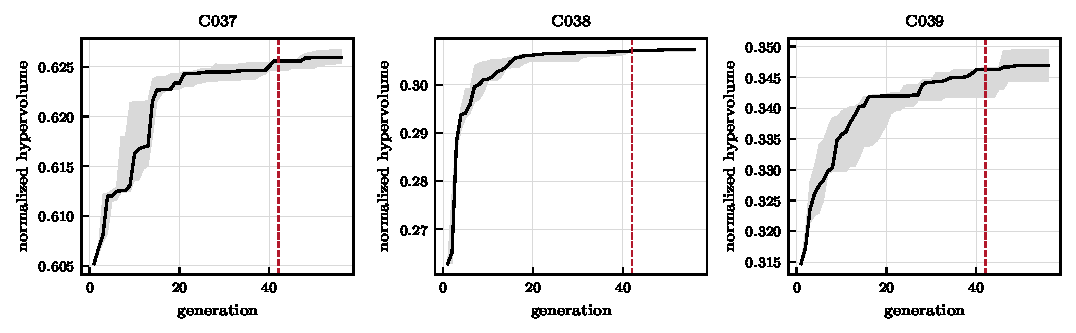
\includegraphics[width=\textwidth]{physics_optimizer_convergence.pdf}
\caption{Median normalized hypervolume over five seeds; shading spans the interquartile range. The dashed line marks generation 42 and all campaigns continue to generation 56. References are fixed within cases.}
\label{fig:physics_optimizer_convergence}
\end{figure}

\begin{table}[t]
\centering\small
\caption{Seed-level optimizer convergence using a fixed hypervolume reference for each case. Gains compare generation 42 with generation 56.}
\label{tab:optimizer_convergence}
\begin{tabular}{lrrrr}
\toprule
Case & Seeds & Mean final HV & Median gain & Maximum gain \\
\midrule
C037 & 5 & 0.6201 & 0.059\% & 0.232\% \\
C038 & 5 & 0.3397 & 0.062\% & 0.126\% \\
C039 & 5 & 0.3596 & 0.541\% & 1.284\% \\
\bottomrule
\end{tabular}
\end{table}


\FloatBarrier
\section{Dimensionless Pareto results}

\subsection{FEM-rebuilt fronts}

The 15 searches produce 540 terminal particles. Merging them with the 80 FEM geometries gives 732 unique case--vector classifications and 572 unique mechanical geometries. All 572 complete their mesh-24 paths. Table~\ref{tab:physics_front_summary_fast} gives the direct objective ranges and member counts after float-safe mechanical reconstruction. These are nondominated sets over this pooled 572-geometry universe, not globally complete fronts over the continuous design domain. Figure~\ref{fig:physics_fronts} overlays every successful, case-feasible direct classification, the resulting sets, and the nine selected representatives.

\begin{table}[t]
\centering
\caption{Direct-FEM nondominated sets over the pooled candidate universe, reconstructed from the complete 24-element ledger.}
\label{tab:physics_front_summary_fast}
\begin{tabular}{lrlrlr}
\toprule
Case & Members & Coordinate 1 & Range & Coordinate 2 & Range \\
\midrule
C037 & 58 & $\phi_b$ & 0.1308--0.2623 & $1/\Psi_U$ & 271.1--1748 \\
C038 & 31 & $\phi_b$ & 0.1308--0.1802 & $\Omega_8$ & 0.4272--0.4721 \\
C039 & 121 & $1/\Psi_U$ & 390.3--3470 & $\Omega_8$ & 0.3487--0.7379 \\
\bottomrule
\end{tabular}
\end{table}


\begin{figure}[t]
\centering
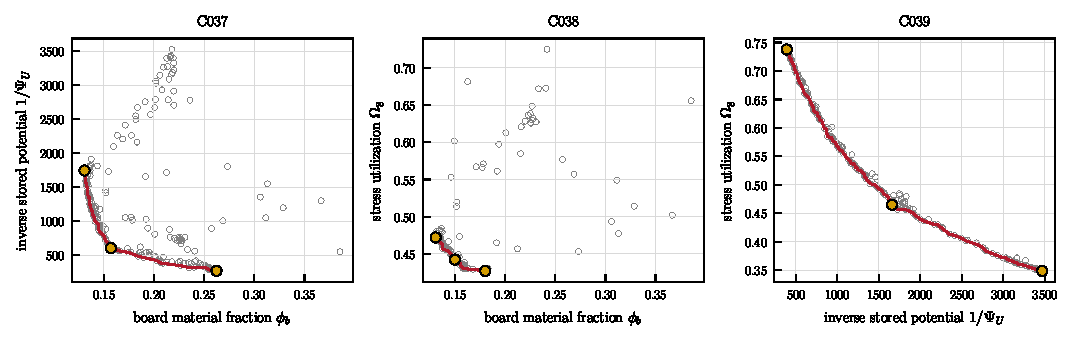
\includegraphics[width=0.98\textwidth]{physics_pareto_fronts.pdf}
\caption{Dimensionless direct-FEM results at 24 elements per period over the pooled candidate universe. Open grey circles are successful case-feasible classifications, red curves are reconstructed nondominated sets, and gold markers are the two extremes and normalized compromise selected in each case.}
\label{fig:physics_fronts}
\end{figure}

C037 spans the broad material--potential exchange: increasing board material fraction can raise stored potential strongly, but the gain is neither proportional nor determined by thickness alone. Crown width, transition curvature, and contact path distinguish designs with similar $\phib$.

C038 intersects the potential floor in a narrow material--stress band. Its 31 direct members span $\phib=0.1308$--$0.1802$ and $\Om=0.4272$--$0.4721$. Because this range is narrow, the C038 extremes and compromise are all included in the nine mesh-32 checks rather than inferring numerical stability from surrogate rank.

C039 is especially informative because its material cap admits profiles with comparable material accounting but very different potential and stress responses. Global material fraction therefore cannot identify the preferred local compression mechanism.

The constraint thresholds are training-defined modelling choices rather than universal material constants. Table~\ref{tab:threshold_sensitivity_fast} rebuilds the strict mesh-24 nondominated sets at nearby quantiles without rerunning mechanics. C038 changes from 49 to 7 members as the stored-potential floor moves from the 30th to the 50th training percentile; C039 changes from 81 to 122 members as the material cap moves from the 55th to the 75th percentile. The nominal 40th and 65th percentiles remain the predeclared cases used elsewhere.

\begin{table}[t]
\centering\small
\caption{Dependence of the strict mesh-24 nondominated sets on nearby training-defined constraint quantiles.}
\label{tab:threshold_sensitivity_fast}
\begin{tabular}{lrrrr}
\toprule
Case & Training quantile [\%] & Threshold & Feasible & Members \\
\midrule
C038 & 30 & 0.000364866 & 183 & 49 \\
C038 & 40 & 0.000455471 & 129 & 31 \\
C038 & 50 & 0.000563887 & 60 & 7 \\
C039 & 55 & 0.21303 & 135 & 81 \\
C039 & 65 & 0.217537 & 210 & 121 \\
C039 & 75 & 0.219906 & 217 & 122 \\
\bottomrule
\end{tabular}
\end{table}


\subsection{Surrogate decision fidelity}

Table~\ref{tab:decision_fidelity_fast} compares screening objectives with direct FEM over every successful, case-feasible mesh-24 classification. In C037 and C038 the first objective is exact geometry, hence its correlation is one and its error is zero. Mechanical rank fidelity is the relevant quantity for optimization, and the C039 stress objective has a 9.56\% median relative error despite a Spearman correlation of 0.953. These results show why the red fronts in Fig.~\ref{fig:physics_fronts} cannot be replaced by the surrogate screen.

\begin{table}[t]
\centering
\caption{Surrogate-to-direct decision fidelity over feasible mesh-24 classifications. $\rho_s$ is Spearman correlation and MARE is median absolute relative error.}
\label{tab:decision_fidelity_fast}
\begin{tabular}{lrrrrr}
\toprule
Case & $n$ & $\rho_{s,1}$ & MARE$_1$ [\%] & $\rho_{s,2}$ & MARE$_2$ [\%] \\
\midrule
C037 & 243 & 1.000 & 0.00 & 0.997 & 2.12 \\
C038 & 129 & 1.000 & 0.00 & 0.957 & 0.98 \\
C039 & 210 & 0.980 & 1.75 & 0.953 & 9.56 \\
\bottomrule
\end{tabular}
\end{table}


\subsection{Representative mesh sensitivity}

Figure~\ref{fig:representative_mesh_verification} and Table~\ref{tab:representative_mesh_convergence} report targeted refinement rather than an all-candidate fine sweep. All nine nondominated-set representatives are paired at 24 and 32 elements; the three case compromises are paired at 32 and 40. Relative change uses the finer-mesh denominator in Eq.~\eqref{eq:mesh_change}. The largest 24--32 relative changes are 0.59\% for $\PsiU$, 0.21\% for $\Om$, and 2.25\% for the raw maximum-stress utilization. Over the accepted 32--40 compromise checks, the corresponding maxima are 0.22\%, 0.088\%, and 1.20\%. The optimized smooth stress number is therefore materially less sensitive than the single-element maximum over this declared sample.

\begin{figure}[t]
\centering
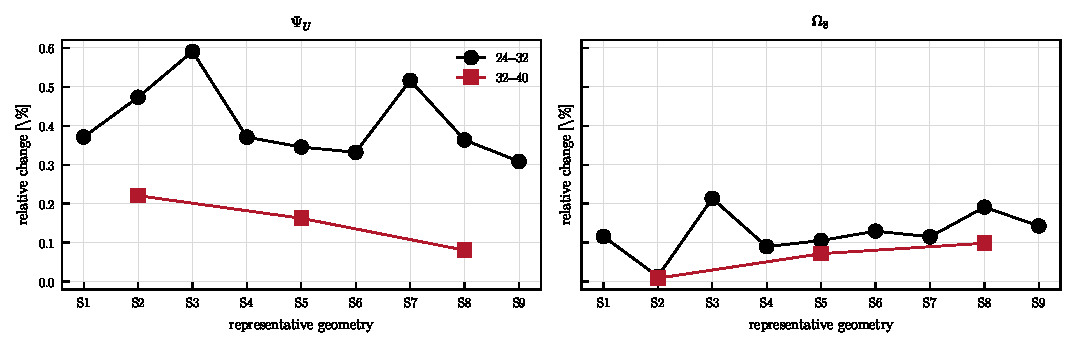
\includegraphics[width=0.96\textwidth]{representative_mesh_convergence.pdf}
\caption{Targeted mesh checks for the nine pooled-candidate nondominated representatives. Circles show 24--32 relative changes; squares show 32--40 changes for the three normalized compromises.}
\label{fig:representative_mesh_verification}
\end{figure}

\begin{table}[t]
\centering
\caption{Relative changes (percent) for representative optimized geometries, using the finer-mesh response as denominator. All nine are checked at 24--32 elements; the three case compromises are also checked at 32--40.}
\label{tab:representative_mesh_convergence}
\begin{tabular}{llrrrr}
\toprule
ID & Case & $\Psi_U^{24\to32}$ & $\Omega_8^{24\to32}$ & $\Psi_U^{32\to40}$ & $\Omega_8^{32\to40}$ \\
\midrule
S1 & C037 & 0.37 & 0.12 & -- & -- \\
S2 & C037 & 0.47 & 0.01 & 0.22 & 0.01 \\
S3 & C037 & 0.59 & 0.21 & -- & -- \\
S4 & C038 & 0.37 & 0.09 & -- & -- \\
S5 & C038 & 0.35 & 0.11 & 0.16 & 0.07 \\
S6 & C038 & 0.33 & 0.13 & -- & -- \\
S7 & C039 & 0.52 & 0.11 & -- & -- \\
S8 & C039 & 0.36 & 0.19 & 0.08 & 0.10 \\
S9 & C039 & 0.31 & 0.14 & -- & -- \\
\bottomrule
\end{tabular}
\end{table}


\subsection{Dimensionless response map}

Figure~\ref{fig:dimensionless_map} maps the FEM dataset and final designs. Aspect ratio and thickness ratio separate families that overlap in material fraction. The map also illustrates why training points were built on feasible local perturbations instead of uniform random samples: manufacturable designs occupy a thin subset of the ten-dimensional box.

\begin{figure}[t]
\centering
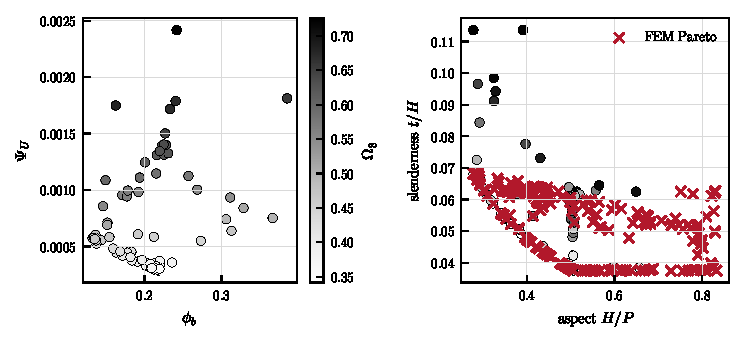
\includegraphics[width=0.86\textwidth]{dimensionless_performance_map.pdf}
\caption{Dimensionless response and design-space maps. The FEM designs establish the response cloud; crosses mark direct-FEM Pareto designs in geometric-ratio coordinates.}
\label{fig:dimensionless_map}
\end{figure}

\FloatBarrier
\section{Optimized geometries and refined simulations}

\subsection{Refined numerical values}

Tables~\ref{tab:selected_physics_designs_fast} and \ref{tab:selected_response_diagnostics_fast} report the two extremes and normalized utopia-nearest compromise from each pooled-candidate nondominated set after the common 32-element check. The three compromises additionally satisfy the strict 40-element path audit. The derived forming-yield index is interpreted separately from service compression: a value above unity means that nominal forming curvature from a flat elastic sheet exceeds the elastic strain scale and therefore requires a forming process or an explicit residual-stress model.

\begin{table*}[t]
\centering\small
\caption{Representative direct-FEM designs at 32 elements per period. $10^3\Psi_U$ is shown for readability.}
\label{tab:selected_physics_designs_fast}
\begin{tabular}{lllrrrr}
\toprule
ID & Case & Role & $R_{\min}$ [mm] & $\phi_b$ & $10^3\Psi_U$ & $\Omega_8$ \\
\midrule
S1 & C037 & objective-1 extreme & 0.901 & 0.131 & 0.570 & 0.472 \\
S2 & C037 & compromise & 0.901 & 0.157 & 1.643 & 0.674 \\
S3 & C037 & objective-2 extreme & 0.900 & 0.262 & 3.667 & 0.781 \\
S4 & C038 & objective-1 extreme & 0.936 & 0.131 & 0.571 & 0.473 \\
S5 & C038 & compromise & 1.021 & 0.150 & 0.491 & 0.443 \\
S6 & C038 & objective-2 extreme & 0.938 & 0.180 & 0.458 & 0.428 \\
S7 & C039 & objective-1 extreme & 0.955 & 0.214 & 2.549 & 0.737 \\
S8 & C039 & compromise & 0.921 & 0.191 & 0.600 & 0.466 \\
S9 & C039 & objective-2 extreme & 0.941 & 0.217 & 0.287 & 0.349 \\
\bottomrule
\end{tabular}
\end{table*}


\begin{table*}[t]
\centering\scriptsize
\caption{Dimensionless response diagnostics for the nine mesh-32 representatives.}
\label{tab:selected_response_diagnostics_fast}
\resizebox{\textwidth}{!}{%
\begin{tabular}{lrrrrrrrrr}
\toprule
ID & $C_F$ & $10^3\Psi_W$ & $\Omega_{99}$ & $\Omega_{\max}$ & $\mathcal L_\sigma$ & $\mathcal I_{WMS}$ & $\mathcal C_y$ & $\Theta$ & $f_y$ \\
\midrule
S1 & 0.0144 & 0.565 & 0.589 & 0.589 & 40.88 & 0.0091 & 4.022 & 0.00100 & 0.000 \\
S2 & 0.0299 & 1.606 & 0.842 & 0.842 & 28.14 & 0.0152 & 4.022 & 0.00075 & 0.000 \\
S3 & 0.0633 & 3.585 & 0.969 & 0.969 & 15.29 & 0.0175 & 6.710 & 0.00063 & 0.000 \\
S4 & 0.0144 & 0.566 & 0.589 & 0.589 & 40.85 & 0.0092 & 3.873 & 0.00099 & 0.000 \\
S5 & 0.0140 & 0.487 & 0.551 & 0.551 & 39.44 & 0.0073 & 3.548 & 0.00106 & 0.000 \\
S6 & 0.0147 & 0.455 & 0.535 & 0.536 & 36.39 & 0.0059 & 3.988 & 0.00119 & 0.000 \\
S7 & 0.0466 & 2.496 & 0.917 & 0.917 & 19.67 & 0.0158 & 5.253 & 0.00092 & 0.000 \\
S8 & 0.0210 & 0.601 & 0.591 & 0.591 & 28.16 & 0.0067 & 4.705 & 0.00211 & 0.000 \\
S9 & 0.0115 & 0.287 & 0.441 & 0.441 & 38.28 & 0.0038 & 3.853 & 0.00103 & 0.000 \\
\bottomrule
\end{tabular}}
\end{table*}


The study-defined combined selector $\Iws$ favors external work relative to both material fraction and smooth stress utilization. It is useful for shortlisting among already nondominated designs but is not a universal utility function and is not used to reconstruct a front.

\subsection{Deformed fields and load paths}

Figure~\ref{fig:stress_gallery} shows the three normalized compromises at the accepted 40-element refinement. Stress is distributed over the deformed centreline rather than inferred from undeformed curvature. Profiles with similar global material fractions can have different local distributions, demonstrating the value of retaining the complete decision vector and the simulated field.

\begin{figure}[p]
\centering
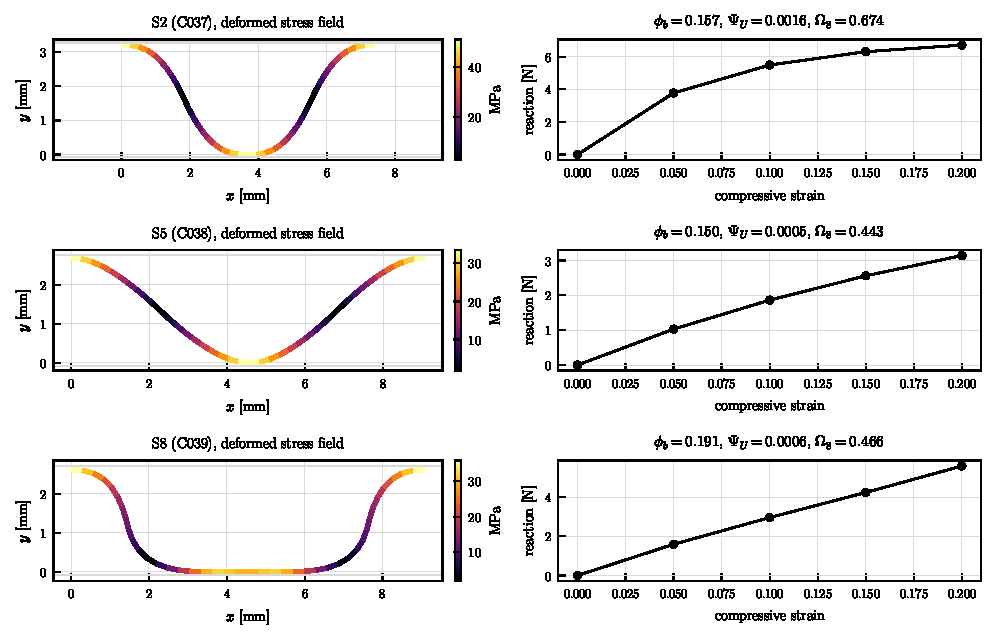
\includegraphics[width=0.98\textwidth]{optimized_fem_stress_gallery.pdf}
\caption{Deformed extreme-fibre stress fields and reaction paths at the 40-element mesh for the C037, C038, and C039 normalized compromises. Line color is the element maximum absolute stress; horizontal grey lines are rigid surfaces at 20\% compression.}
\label{fig:stress_gallery}
\end{figure}

Reaction curves are evaluated over the complete declared path and can exhibit different tangent evolution. A positive refined last-interval tangent $\Theta$ supports local monotonic response along the sampled compression coordinate, but it is not a two-coordinate Hessian test and does not exclude unsampled bifurcations.

The smooth $p$-norm is retained as the optimized stress variable because it is less mesh-sensitive than a single extreme. The length-weighted $\Omega_{99}$ and raw $\Ommax$ values are still reported so averaging cannot hide local stress. The targeted changes in Fig.~\ref{fig:representative_mesh_verification} establish numerical resolution for the selected designs rather than experimental stress accuracy or asymptotic convergence of every front member.

\subsection{Computational cost}

Table~\ref{tab:runtime_summary_fast} reports measured complete-path runtimes for the 80 training geometries, the already completed 572-geometry coarse reconstruction, the nine mesh-32 representatives, and the three mesh-40 compromises. Counts refer to unique mechanics solves rather than repeated case classifications. The targeted refinement adds 12 accepted paths instead of the 1072 extra paths required by the discarded all-candidate 32/40/48 plan. The table also discloses the three rejected exploratory mesh-48 paths: they consumed 316.0 CPU-process seconds and are excluded from the evidence.

\begin{table}[H]
\centering
\caption{Measured complete-path FEM cost. Times are CPU-process seconds in the x86--64 container on an Intel Xeon Platinum 8573C; representative batches use at most three processes. Accepted evidence rows are followed by an excluded solver-audit row.}
\label{tab:runtime_summary_fast}
\begin{tabular}{lrrrrr}
\toprule
Ledger & Mesh & Paths & Sum [s] & Median [s] & Max [s] \\
\midrule
Training & 16 & 80 & 412.4 & 4.73 & 13.22 \\
Coarse reconstruction & 24 & 572 & 4296.4 & 7.23 & 18.36 \\
Representatives & 32 & 9 & 271.9 & 15.69 & 100.30 \\
Case compromises & 40 & 3 & 375.7 & 119.69 & 137.73 \\
Rejected audit (excluded) & 48 & 3 & 316.0 & 88.31 & 139.47 \\
\bottomrule
\end{tabular}
\end{table}


The runtime distribution is geometry dependent because contact activation, bounds, and nonlinear iterations vary by shape. Evaluation count remains the appropriate optimizer budget, while elapsed time remains useful for planning mechanical verification. Neural query time is not compared with FEM path time here because the scientific decision includes geometric screening, uncertainty evaluation, and subsequent direct solution rather than a single isolated forward call.

\FloatBarrier
\section{Discussion}

\subsection{What changes when nonlinear mechanics is optimized}

The geometric benchmark finds a narrow area--inertia band, but the mechanical fronts cover broad potential and stress ranges. Global inertia cannot uniquely encode platen contact sequence, axial/bending partition, local yielding regularization, or shape-dependent lateral contraction. Nonlinear results do not invalidate geometric screening; they show where it ceases to be sufficient.

Pitch and height often move to bounds, but not in one universal direction. Low-material members favor large $P$, large $H$, and minimum $t$ because bounding rectangle and liner proxy dominate $\phib$. High-potential members shorten pitch or increase thickness, raising reaction and stored potential. Stress-limited members can instead alter rational crown shape and transition length while keeping thickness near its lower bound. This distinction is visible across the selected representatives and would be obscured by optimization over $t$ alone.

The radius threshold is active or nearly active for several extremes, as quantified for every representative in Table~\ref{tab:selected_physics_designs_fast}. These designs satisfy the deterministic model but leave little manufacturing margin. A production study should replace the nominal threshold with a robust condition, for example $\Pr(\Rmin<0.9)\le\alpha$, using tool, thickness, moisture, and spring-back distributions. The present pooled-candidate nondominated set is a nominal mechanical envelope.

\subsection{Role of the neural model}

The dimensionless formulation supports neural generalization because potential is learned after division by $\sigma_ybtL_s$, and conjugate force is scaled consistently. The held-out errors are adequate for in-domain search guidance, but the narrow C038 stress band remains a demanding rank problem. High $R^2$ and low mean error therefore do not justify reporting neural optima as mechanical optima.

Complete mesh-24 re-simulation of the terminal population addresses within-population selection bias, while adding all training geometries prevents the optimizer endpoints from defining the entire direct comparison set. The neural layer saves search cost by focusing on promising, in-domain regions; FEM supplies the numbers and classifications used in claims. The decision-fidelity table is as important as the prediction plot because optimization uses order and feasibility, not only mean squared error. Targeted 32/40 refinement supports the reported representatives but does not certify the discretization error or membership of every one of the 210 coarse nondominated members. This verification also cannot exclude an undiscovered design outside the combined sampled regions.

Stress deserves a separate warning. The energy surrogate does not predict local stress, and the auxiliary ensemble does not inherit energy conjugacy. Its purpose is to prioritize regions. Direct FEM $\Om$, $\Omega_{99}$, and $\Ommax$ replace it after screening. A future stress-aware neural operator would require local-field supervision, mesh-independent coordinates, and validation spanning topology and contact states.

\subsection{Interpretation of the dimensionless numbers}

The eight-entry independent basis in Eq.~\eqref{eq:input_groups} and the responses in Eqs.~\eqref{eq:load_number}--\eqref{eq:localization_tangent} separate scale and mechanism more cleanly than arbitrary multipliers on area, stiffness, or energy. The identities $\tau_P=\eta\tau_H$ and $\mathcal C_y=(E/2\sigma_y)\Pi_\kappa$ prevent derived quantities from being counted as additional inputs. $\phib$ expresses board material accounting, whereas $\phic$ isolates the mechanically simulated medium. $\PsiU$ and $\PsiW$ remain distinct: they are close under the present conservative regularization, but the distinction becomes essential with friction, damage, or irreversible plasticity.

$\mathcal C_y$ connects manufacturability and material scale. Values above one indicate that forming cannot be interpreted as purely elastic bending. $\mathcal L_\sigma$ distinguishes local stress concentration from nominal crush load. Finally, $\mathcal I_{WM}$, $\mathcal I_{WS}$, and $\Iws$ provide compact selectors without expanding Pareto dimension. Their value is comparative within the declared protocol, not universal across materials, strains, or boundaries.

\subsection{Physical scope and limitations}

The following boundaries apply:
\begin{enumerate}[leftmargin=*,itemsep=3pt]
\item FEM represents a single pre-formed medium between rigid surfaces with a $t/2$ centreline-to-surface offset, prescribed normal motion at the trough and periodic crowns, and free tangential slip. Flexible liners, adhesive constitutive response, friction, and debonding are omitted.
\item The smooth yielding law is a deformation potential. It does not model path-dependent damage, hysteresis, crushing dissipation, moisture effects, or irreversible fibre-network evolution.
\item Material constants are fixed. The study establishes relative performance within that model and does not claim experimental strength for new geometries.
\item The path is monotonic compression to 20\%. Unloading, repeated loading, deeper self-contact, and package-scale boundary effects are outside scope.
\item Scalar tangent $\Theta$ is not a complete stability analysis. Imperfection-sensitive bifurcation and coupled pitch--compression tangent require extra coordinates and branch tracking.
\item The 0.9~mm radius condition is deterministic. No tooling tolerance or process-capability distribution is included.
\item Direct FEM reconstruction validates surrogate decision fidelity against the same model that generated training data. The complete front uses mesh 24; the 32/40 checks apply only to the declared representatives and are not a claim of asymptotic convergence or universal membership stability.
\end{enumerate}

These limits define the level of the result. The reported sets are numerically verified trade-offs over the declared pooled candidates for one explicit periodic model, suitable for choosing a compact set of specimens for forming and experimental flat-crush evaluation.

\section{Conclusions}

A geometric corrugated-board optimization has been extended to nonlinear, stress-aware, dimensionless multi-objective design. The main conclusions are:
\begin{enumerate}[leftmargin=*,itemsep=3pt]
\item A ten-variable rational NURBS model supports coupled pitch, height, thickness, and shape search while enforcing a physical 0.9~mm radius threshold.
\item A minimal independent dimensionless basis separates geometry from scale; derived identities are reported explicitly. Response numbers separate board material proxy, core fraction, crush load, stored potential, external work, smooth/local stress, localization, and tangent response. Combined selector $\Iws$ shortlists an existing front without becoming an independent objective.
\item Eighty geometries and 400 accepted FEM states provide an in-domain screen. Held-out full-path tests quantify energy, reaction, and stress error without mixing load states from the same geometry across the split.
\item Neural prediction quality is not treated as proof of optimality. Terminal populations are merged with all FEM designs; all 732 case classifications representing 572 unique geometries receive matched, finite direct mechanics at mesh 24.
\item The reconstructed nondominated sets over the pooled 572-geometry universe contain 58 C037, 31 C038, and 121 C039 members. Nine extremes/compromises pass mesh 32, and the three case compromises pass mesh 40; the maximum representative changes in $\PsiU$ and $\Om$ remain below 0.6\% and 0.22\%, respectively, on the declared intervals.
\item Similar material fractions can support sharply different mechanics because profile shape changes the contact sequence, axial--bending partition, and stress localization.
\item Representative optimized geometries are reported with complete ten-variable vectors, direct response diagnostics, targeted mesh changes, and accepted 40-element deformed stress fields for the three case compromises.
\end{enumerate}

The immediate next physical step is to manufacture a set spanning material, potential, stress, and combined-selector extremes, then calibrate flexible-liner/contact and imperfection parameters against full load paths rather than isolated terminal values.

\section*{Code and data availability}

The complete manuscript source, optimization code, FEM implementation, trained-model parameters, numerical ledgers, figures, generated tables, tests, and execution manifests are maintained at \url{https://github.com/rfitas-lab/corrugated-board-size-shape-optimization}. The immutable source-and-data commit associated with the final article is linked from the compiled manuscript. Every numerical claim is generated from files included in that reproducibility package. Superseded exhaustive-protocol outputs are quarantined under \path{project/legacy_exhaustive_protocol} and are excluded from the fast manifest. The three rejected mesh-48 attempts are retained as a solver audit but are not inputs to any reported nondominated set, table, figure, or conclusion.

\appendix

\section{Experiment family taxonomy}

The case identifiers distinguish parameterizations and objective families; they are not a chronological claim. Table~\ref{tab:case_taxonomy} gives the interpretation used in this paper. C001--C033 explore size-only or shape-only dimensionality, C034--C036 couple size and shape with geometric/linear quantities, and C037--C039 are the nonlinear dimensionless cases introduced here.

\begin{table}[H]
\centering\small
\caption{Optimization experiment families.}
\label{tab:case_taxonomy}
\begin{tabularx}{\textwidth}{lllX}
\toprule
Cases & Variables & Count & Primary role \\
\midrule
C001--C004 & layer thicknesses, pitch, height & 5 & size-only board studies \\
C005--C008 & pitch and height & 2 & reduced size trade-offs \\
C009--C011 & four shape control points & 13 & low-order free-form shapes \\
C012--C014 & eight shape control points & 25 & intermediate free-form shapes \\
C015--C017 & fifteen shape control points & 46 & high-dimensional shape study \\
C018 & compact rational profile & 7 & reduced NURBS representation \\
C019--C027 & 4/8/15-point production families & 13/25/46 & parameterization comparison \\
C028--C030 & compact rational profile & 7 & objective-pair comparison \\
C031--C033 & compact rational profile & 7 & radius-constrained benchmark \\
C034--C036 & compact shape plus $P,H,t$ & 10 & geometric coupled size--shape study \\
C037--C039 & compact shape plus $P,H,t$ & 10 & dimensionless FEM/neural-screen optimization \\
\bottomrule
\end{tabularx}
\end{table}

The progression in variable count clarifies a recurring design trade-off. A high-dimensional control-point representation can express more local features but produces more degeneracy and a thinner feasible region. The compact rational representation encodes periodic topology and uses weights to control transition sharpness. Coupling it to $P$, $H$, and $t$ then changes both geometric scale and mechanical slenderness without introducing dozens of independent coordinates.

\section{Complete rational B-spline definition}

For degree $p$, the Cox--de Boor basis is
\begin{align}
N_{i,0}(u)&=\begin{cases}
1,&u\in[\xi_i,\xi_{i+1}),\\
0,&\text{otherwise},
\end{cases}\\
N_{i,p}(u)&=\frac{u-\xi_i}{\xi_{i+p}-\xi_i}N_{i,p-1}(u)
+\frac{\xi_{i+p+1}-u}{\xi_{i+p+1}-\xi_{i+1}}N_{i+1,p-1}(u),
\end{align}
where a zero denominator contributes zero. With ten control points and $p=2$, the clamped knot vector has three repeated end knots and uniformly spaced internal knots. The repeated control construction places exact crowns at $u=1/4$ and $3/4$ and a trough at $u=1/2$; the mechanical period is always the inclusive crown-to-crown interval. Physical $x$ and $y$ are scaled independently to $P$ and $H$ after extraction.

The manufacturing evaluator uses a dense parameter grid because second numerical gradients are sensitive to sampling. The FEM grid interpolates physical $(x,y)$ in cumulative arc length within segments divided by exact trough and crown nodes. Thus radius is not inferred from the coarse beam mesh, near-vertical segments are not erased by $x$-sorting, and contact extrema are present at every resolution.

\section{Geometric benchmark objective conventions}

The geometric benchmark uses physical reports
\begin{align}
A_P&=A/P\quad[\mathrm{mm}],\\
I_P&=I/P\quad[\mathrm{mm^3}],\\
E_{z,\mathrm{eff}}&\quad[\mathrm{MPa}],\\
R_1,R_2&\quad[\mathrm{mm}].
\end{align}
Optimization coordinates are declared as minimization. Minimizing $1/I_P$ is equivalent to maximizing $I_P$, but plotted axes retain physical increasing direction. Hypervolume depends on scaling and reference point; physical front coordinates are the reusable engineering result.

Corrected dominance is
\begin{equation}
\bm f_i\preceq\bm f_j
\quad\text{and}\quad
\exists k:f_{ik}<f_{jk},
\end{equation}
after both quantities are minimization. Feasible points constraint-dominate infeasible points; infeasible points are ordered by total violation; feasible points use Pareto dominance and crowding.

\section{Mechanical post-processing details}

At each element, axial strain and curvature are recovered from current chord and relative rotations. Four extreme-fibre stresses are evaluated: top and bottom at both element ends. Their maximum absolute value defines $\sigma_e$ in Eq.~\eqref{eq:stress_pnorm}. The length-weighted quantile is found by sorting $\sigma_e$ and accumulating $L_e$ rather than counting elements, preventing local refinement from changing a percentile merely by adding short elements.

Yielded-length fraction is
\begin{equation}
f_y=\frac{\sum_eL_e\,\mathbf 1(\sigma_e\ge\sigma_y)}{\sum_eL_e}.
\end{equation}
It is evaluated for every accepted mesh-32 representative and mesh-40 compromise under the smooth law and target strain. A low or zero value under this nominal path does not exclude yielding after deeper compression or with geometric imperfections.

Stored potential and external work are monitored independently. With displacement control, no friction, and a smooth conservative material potential, they should remain close. Table~\ref{tab:solver_audit_fast} documents the accepted paths and solver fallbacks; the potential--work difference results from five-point trapezoidal reaction integration and solver tolerance. Neither is labeled dissipated energy.

\section{Full selected design vectors}

\begin{table}[H]
\centering\scriptsize
\caption{Complete ten-variable vectors for the representative designs.}
\label{tab:selected_design_vectors}
\resizebox{\textwidth}{!}{%
\begin{tabular}{llrrrrrrrrrr}
\toprule
ID & Case & $x_1$ & $x_2$ & $x_3$ & $x_4$ & $x_5$ & $x_6$ & $x_7$ & $P$ & $H$ & $t$ \\
\midrule
S1 & C037 & 0.10000 & 10.00000 & 10.00000 & 10.00000 & 9.37702 & 0.00000 & 0.00000 & 7.90000 & 4.00000 & 0.15000 \\
S2 & C037 & 9.96769 & 0.10000 & 10.00000 & 0.10000 & 0.10000 & 0.00000 & 0.00000 & 4.80000 & 4.00000 & 0.15000 \\
S3 & C037 & 10.00000 & 0.10000 & 10.00000 & 0.10000 & 0.10000 & 0.00000 & 0.00000 & 4.80000 & 3.98618 & 0.25000 \\
S4 & C038 & 0.58927 & 8.96259 & 9.48083 & 9.99523 & 8.63075 & 0.00000 & 0.00000 & 7.90000 & 4.00000 & 0.15001 \\
S5 & C038 & 0.10000 & 9.60499 & 8.69185 & 10.00000 & 8.70160 & 0.00000 & 0.00000 & 7.90000 & 3.36604 & 0.15000 \\
S6 & C038 & 1.17359 & 9.50789 & 6.77285 & 6.75565 & 6.21128 & 0.00000 & 0.14019 & 7.78700 & 2.81642 & 0.15479 \\
S7 & C039 & 10.00000 & 0.10000 & 10.00000 & 0.10000 & 0.10000 & 0.00000 & 0.00000 & 5.04698 & 4.00000 & 0.20772 \\
S8 & C039 & 9.80191 & 0.10416 & 8.64012 & 0.10179 & 10.00000 & 0.00500 & 0.01832 & 7.90000 & 3.27331 & 0.17932 \\
S9 & C039 & 3.03892 & 10.00000 & 7.31343 & 10.00000 & 10.00000 & 1.00000 & 1.00000 & 7.90000 & 2.20000 & 0.15000 \\
\bottomrule
\end{tabular}}
\end{table}


The first five entries $x_1,\ldots,x_5$ in Table~\ref{tab:selected_design_vectors} are raw positive spacing variables; the normalized coordinates in the NURBS definition are $d_i=x_i/\sum_jx_j$. Another vector obtained by multiplying all five raw values by a common positive constant represents the same curve. The next entries $x_6,x_7$ are bounded parameters mapped to the rational factors by Eq.~\eqref{eq:weight_mapping}. The printed table rounds coordinates to five decimal places for readability; the full-precision vectors in \texttt{selected\_optimized\_geometries.csv} reproduce the reported designs.

\section{Optimization failure handling}

For an infeasible or failed candidate, the callback returns finite objective values and continuous violation
\begin{equation}
v=v_R+v_D+v_{\mathrm{case}}+v_{\mathrm{solve}},
\end{equation}
where $v_R$ is normalized radius violation, $v_D$ is excess trust distance, $v_{\mathrm{case}}$ is C038 energy or C039 material violation, and $v_{\mathrm{solve}}$ is positive for a failed path. This prevents exceptions or NaNs from entering nondominated sorting. Reported set members require $v=0$, a matched successful mesh-24 mechanics record, finite direct objectives, and exact within-case nondominated membership over the pooled candidate universe. Representative refinement is reported separately and does not retroactively change coarse-set membership.

The seeded swarm retains an unseeded mode as default; physics cases supply feasible initial positions and reduced velocity scale. Bounds are enforced after every update. Parent and trial particles are combined, ranked by constraint-compatible fronts, and truncated by normalized crowding. Personal bests update under constraint domination; mutually nondominating ties are broken stochastically.

\section{Numerical checklist}

\begin{enumerate}[leftmargin=*,itemsep=2pt]
\item verify NURBS invariance under common scaling of $x_{1:5}$;
\item evaluate 800-sample physical radius before a design enters the feasible pool;
\item split by geometry, never by load-state row;
\item insert exact crown/trough nodes and verify zero initial contact gaps at every mesh;
\item store every FEM state, raw status, projected gradient, reaction balance, terminal metric, and runtime;
\item train five energy-consistent neural potentials and evaluate the geometry-held-out design split;
\item report additive stress residual calibration descriptively and serialize the neural ensembles, tree model, scaler, and neighbor model;
\item construct trust limit from training leave-one-out distances only;
\item run all cases and seeds with the same budget;
\item merge terminal and training designs, solve each of the 572 unique geometries once at 24 elements, join by a rounded coordinate key, and reclassify raw mechanics by case;
\item select two extremes and one normalized compromise per case, then verify all nine unique representatives at 32 elements;
\item refine the three case compromises at 40 elements and reject any path that fails the predeclared solver criterion;
\item fingerprint the protocol, ordered ledgers, thresholds, and classification rules before reusing results;
\item generate tables and figures from direct numerical values.
\end{enumerate}

\section{Scaling, robustness, and experimental extension}

If all in-plane lengths and thickness are scaled by a common factor $s$ while $b$, $E$, and $\sigma_y$ remain fixed, then $L_s$, $P$, $H$, and $t$ scale with $s$. The fractions $\phic$, $\phib$, $\eta$, $\tau_H$, and $\Pi_\kappa$ are invariant; $\tau_P$ follows from $\eta\tau_H$. The normalizers in Eqs.~\eqref{eq:load_number}--\eqref{eq:work_number} remove the leading section and path scales. Exact response invariance is not guaranteed because the beam/contact idealization and smooth yielding law retain geometry-dependent effects. The dimensionless formulation is therefore a similarity organization, not an assertion that all scaled cells are mechanically identical.

A robust continuation can introduce uncertain vector $\bm\omega$ containing thickness, forming-radius bias, pitch, height, modulus, and yield stress. One possible formulation is
\begin{align}
\min_{\bm x}\quad &\left(
\mathbb E[\phib],
-\mathbb E[\PsiW],
Q_{0.95}[\Om]
\right),\\
\text{subject to}\quad
&\Pr[\Rmin(\bm x,\bm\omega)<0.9]\le\alpha,\\
&\Pr[\Theta(\bm x,\bm\omega)\le0]\le\beta.
\end{align}
This extension should not be performed with arbitrary probability distributions. Tool measurements, formed-profile scans, and paper-property tests are needed to identify $\bm\omega$ and its correlations.

The selected geometries define a compact experimental matrix spanning the two extremes and normalized compromise of each material--potential, material--stress, and potential--stress front, with duplicate geometries tested only once. The combined selector provides an additional cross-case shortlist without changing Pareto membership. At minimum, tests should record the complete reaction--displacement path, formed geometry before loading, contact sequence, and failure location. Repeated specimens are needed to distinguish geometry trends from paper and forming variability.

Calibration should use pathwise quantities rather than one terminal force. Suitable targets include reaction at each strain, initial contact strain, tangent changes, final deformed ordinates, and full-field strain where available. Model validation should then reserve at least one geometry family and one thickness level not used in calibration. Only after that step would it be defensible to interpret $\PsiW$ as a validated design quantity rather than a numerically consistent mechanical index.

\FloatBarrier

\bibliographystyle{unsrtnat}
\bibliography{../references}

\end{document}
